\documentclass[12pt]{report}

\usepackage{pdfpages}

\usepackage{graphicx}
\graphicspath{ {figures/} }
\graphicspath{{images/}}
\usepackage[margin=1 in, includefoot]{Geometry}
\usepackage{hyperref}
\hypersetup{colorlinks=true,linkcolor=blue,urlcolor=cyan,}
%pdfpagemode=fullScreen}
\usepackage[english]{babel}
\usepackage[utf8]{inputenc}
\usepackage{fancyhdr}
\pagestyle{fancy}
\fancyhf{}
\renewcommand{\headrulewidth}{0pt}
\renewcommand{\footrulewidth}{1pt}
\usepackage{ragged2e}
\usepackage{times}
\usepackage{array}
\renewcommand\thesection{\arabic{section}}
\usepackage {hyperref}
\usepackage{graphicx,wrapfig,lipsum}
\usepackage{array}
\usepackage{multirow}

\DeclareUnicodeCharacter{0394}{\ensuremath{\Delta}}

%header and footer
\cfoot{\fontsize{10}{12} \selectfont DYPIT, Department of Computer Engineering 2022-2023 }
%\chead{Cloud Cryptography: User End Encryption}




\begin{document}

%Start of Title page

\centering \large \textbf  {A PRELIMENERY REPORT ON   }\\
\vspace{0.9 cm}
\Large \textbf{"PC Game Development using Unity”}\\
\vspace{0.5 cm}
%\normalsize {on}\\
%\vspace{0.1 cm}
\normalsize{SUBMITTED TO THE SAVITRIBAI PHULE PUNE UNIVERSITY, PUNE}\\
\normalsize{IN THE PARTIAL FULFILLMENT OF THE REQUIREMENTS}\\
\normalsize{  FOR THE AWARD OF THE DEGREE}\\
\vspace{0.8 cm}
\normalsize {Of}\\
\vspace{0.8 cm}

\Large\textbf{BACHELOR OF COMPUTER ENGINEERING}\\
\vspace{0.9 cm}
\large{SUBMITTED BY}\\
\vspace{0.3 cm}

\large \textbf  {Ankur Patil (BCOB10)}

\large \textbf  {Lalu Nair (BCOB05) }

\large \textbf{Viren Patil (BCOB14)}

\large \textbf{Sharan Thakur (BCOB09)}
%\vspace{0.3 cm}


\begin{figure}[h]
\centering

\includegraphics[scale=0.25]{Logo.png }
\end{figure}

\centering \Large \textbf  {DEPARTMENT OF COMPUTER ENGINEERING}\\
\vspace{0.4cm}

\large \textbf  {DR. D. Y. PATIL INSTITUTE OF TECHNOLOGY}\\
\normalsize {PIMPRI, PUNE 411018}\\
\vspace{0.2 cm}
\large \textbf{SAVITRIBAI PHULE PUNE UNIVERSITY}\\


\large \textbf  {2022-2023}\\
\vspace{0.5 cm}

\clearpage
% End of Title page

% start of Certificate

%\begin{wrapfigure}{l}{5.5cm}
\begin{figure}[h]
\centering

\includegraphics[width=6cm]{Logo.png}
%\end{wrapfigure} 
\end{figure}

\vspace{0.3 cm}
\centering{\large \textbf{CERTIFICATE}\\}

\vspace{0.4 cm}

\normalsize{This is to certify that the Project Entitled}\\
\vspace{0.3cm}
\large\textbf{PC Game Development using Unity}\\
\vspace{0.3 cm}
\normalsize{Submitted by}\\
\vspace{0.3 cm}

\normalsize  {Ankur Patil (BCOB10)}

\normalsize  {Lalu Nair (BCOB05)}

\normalsize  {Viren Patil (BCOB14)}

\normalsize  {Sharan Thakur (BCOB09)}

\vspace{0.2 cm}
\justifying
\setlength{\parindent}{4em}
\setlength{\parskip}{1em}
\renewcommand{\baselinestretch}{1.5}
\normalsize
are bonafide students of Dr. D. Y. Patil Institute of Technology and the work has been carried 
out by them under the supervision of Mr. Sharad Adsure (Asst. Professor) and Mrs. 
Deepika Jaiswal (Asst. Professor), it is approved for the partial fulfillment of the 
requirement of Savitribai Phule Pune University, for the award of the degree of Bachelor of Computer
Engineering.

\vspace{0.4 cm}
\setlength{\parindent}{0 em}
 \textbf{Mr. Sharad Adsure}  \hspace{6.9cm}          \textbf{ Dr.Vinod Kimbahune  }   \hspace{5.5cm}         
\centering
(Internal Guide)    \hspace{6.9 cm}  ( Head of the Department)  \hspace{1 cm}    \\

\vspace{0.7 cm}
\setlength{\parindent}{0 em}
\textbf{  External Examiner}   \hspace{7cm}      \textbf    {Mrs.Sunita Patil }   \hspace{5.5cm}         
\centering
.   \hspace{10cm}  ( Project Coordinator)  \hspace{2 cm}    \\
\vspace{0.4cm}
\centering
\textbf{Dr. Lalit Kumar Wadhwa}\\
 Principal,\\
 Dr. D. Y. Patil Institute of Technology,\\
 Pimpri, Pune – 411018
\vspace{0.1 cm}
\begin{flushleft}

Date:
\end{flushleft}


\clearpage


% End of Cerficate


% start of ACKNOWLWDGEMENT

\vspace{4 cm}
\centering{\LARGE \textbf \underline{ACKNOWLEDGEMENT}\\}
\vspace{1 cm}
\justifying
\vspace{1 cm}
\justifying
\setlength{\parindent}{4em}
\setlength{\parskip}{1em}
\renewcommand{\baselinestretch}{1.5}
\normalsize
It gives us great pleasure in presenting the preliminary project report on “PC GAME DEVELOPMENT USING UNITY”


We would like to take this opportunity to thank my internal guides Asst. Prof. Sharad Adsure as well as Ms. Deepika Jaiswal for giving me all the help and guidance we needed. We are really grateful to them for their kind support. Their valuable suggestions were very helpful. 


We are also grateful to Dr. Lalit Kumar Wadhwa, Principal as well as Dr. Vinod V. Kimbahune, Head of Computer Engineering Department, Dr. D.Y Patil Institute Of Technology, Pimpri for his indispensable support, suggestions.


\begin{flushright}

\normalsize  {Ankur Patil (BCOB10)}

\normalsize  {Lalu Nair (BCOB05)}

\normalsize  {Viren Patil (BCOB14)}

\normalsize  {Sharan Thakur (BCOB09)}
\end{flushright}
\clearpage
%end of Acknoledgement
 
% start of ABSTRACT
\vspace{4 cm}
\centering{\LARGE \textbf \underline {ABSTRACT}}\\
\vspace{1 cm}
\justifying
\setlength{\parindent}{4em}
\setlength{\parskip}{1em}
\renewcommand{\baselinestretch}{1.5}
\normalsize
The 2D (Dodgeball Video Game) is a multiplayer game written in Unity 3D using C\#. The game allows players to play over a network, locally with friends on the same network, or over the internet via Photon Cloud. The game plays as you would expect from a dodgeball game. Players can run around, pick up balls, and throw them at each other. If the player is hit enough times, the player is eliminated. Players can choose to continue the game or stop at the end of the game. This game is made with assets and different packages that users can enjoy! This "dodgeball video game" aims to appeal to a market that is still under-tapped. There are already several examples of dodgeball games on the market, but none are perfect and each has some compromises. Some with great interaction with the field, but leave room for variables such as ball/player skill, etc. Proper implementation will keep our users intrigued  and provide a great and unique gaming experience Our main desire is to analyze the existing small market and build on previous dodgeball game attempts to develop a never-before-seen and unique dodgeball experience. Being able to reproduce the game and take advantage of the technology here today will help produce new life into the game dodgeball. Although it will not be 100 percent similar to the original game we all played as kids, the same basic principle of working together as a team to eliminate the enemy team is still present.

\raggedright{ \textbf \underline{KEYWORDS : }}Unity 2D, Game Development, Mono Behaviour, C\#, Real–World, Object Oriented Programming, WEBGL, iOS

\clearpage
% end of  ABSTRACt


% Start of table of content

\tableofcontents
\clearpage
% end of table of content

% Start of table of figures
\listoffigures
\thispagestyle{empty}
\clearpage
\pagenumbering{arabic}
\fancyhead[R]{\thepage}
% end of table of figures

% INTROUDCTION
\centering
\section{INTRODUCTION}
\raggedright
\subsection{OVERVIEW}
\justifying
\setlength{\parindent}{3.7em}
\setlength{\parskip}{0.5em}
\renewcommand{\baselinestretch}{1.5}
\normalsize
\hspace{1.7cm}
This engineering project report details the development of "The Infinite Pleasure", a multiplayer dodgeball video game created using Unity and the Photon Unity extension. The game offers an immersive and interactive experience for players, allowing them to choose their character, map, and compete with friends on the same local network.

The game follows traditional dodgeball rules, with players picking up balls, running around, and throwing them at each other. The game employs a server-client relationship to handle essential concepts such as rendering, player data, and network connectivity.

"The Infinite Pleasure" offers a unique twist to the classic dodgeball game, with innovative gameplay mechanics that would be impossible to replicate in real life. Players are placed into teams, and their objective is to catch, dodge, and launch the ball into the air to eliminate the opposing team.

The game's matchmaking system ensures that players with similar or slightly higher experience levels are paired together. This report outlines the development process, including the game's mechanics design, network architecture, and matchmaking system.

Overall, "DogeBall" combines the fun and chaotic gameplay of dodgeball .With its multiplayer features and Unity integration, it offers an enjoyable and competitive gaming experience for players to engage in virtual doge-themed dodgeball matches.
\clearpage

\raggedright
\subsection{ Motivation}

\justifying
\setlength{\parindent}{4em}
\setlength{\parskip}{0.5em}
\renewcommand{\baselinestretch}{1.5}
\normalsize\hspace{1.7cm}\begin{itemize} \item We are living at the cusp of modern technology with pocket computers with us (our smartphones), in our leisure time, all of us reach into our smartphones to play the next big game to pass time.

\item Being the students we are and wanting to play the latest and greatest games; which drives us to build a unique mechanic for the multiplayer systems.

\item A game is much more than just its software. It has to provide a much more enjoyable experience.

\item Not enough good dodgeball games free-to-play.\\
\end{itemize}
\raggedright
\subsection{Problem Definition}

\justifying
\setlength{\parindent}{4em}
\setlength{\parskip}{0.5em}
\renewcommand{\baselinestretch}{1.5}
\normalsize \hspace{1.7cm} The lack of engaging and interactive multiplayer games for PC users has resulted in a gap in the market and limited options for entertainment. The need for a fun and challenging multiplayer game that can be played on PC has been identified, with the goal of providing an enjoyable and unique gaming experience for users.

In this problem definition, the identified issue is the lack of engaging multiplayer games for PC users, which presents an opportunity to develop a new game that can fill this gap in the market. This sets the stage for the project's objectives, such as developing a multiplayer dodgeball game using the Unity Game Engine for PC, to address this problem and provide a new and enjoyable gaming experience for users.
\clearpage
\raggedright
\subsection{Project Scope And Limitations }
\subsubsection{Project Scope}
\justifying
\setlength{\parindent}{2em}
\setlength{\parskip}{0.5em}
\renewcommand{\baselinestretch}{1.5}
\normalsize \hspace{1.7cm} The Project Scope for our multiplayer dodgeball game using the Unity Game Engine for PC includes the following features that will be implemented in the future to enhance the game's overall effectiveness, efficiency, and success:

i. Porting the game to phones (iOS A Android) and deploying it on App Store and Play Store to reach a wider audience.

ii. Implementing a health system as a mode for a match, which will add a new layer of complexity to the game and make it more challenging for players.

iii. Adding power-ups for players to choose from, which will give players temporary advantages over their opponents, adding a new strategic element to the game.

iv. Adding player-specific buffs that can be purchased, which will allow players to customize their characters and give them an advantage in the game.

v. Adding In-App Purchasing using Unity IAP features, which will allow players to purchase additional features or upgrades within the game, generating additional revenue for the project.

vi. Enhancing gamepad integrations, which will make the game more accessible to players who prefer using gamepads over keyboard and mouse controls.

These features are not included in the current project scope but are essential for the game's future success. The project team will carefully consider each feature's feasibility, resource requirements, and potential impact on the project's timeline, budget, and deliverables before implementing them. The project team will also consult with key stakeholders to ensure that the new features align with the project's overall goals and objectives.

\subsubsection{Limitations}
\justifying
\setlength{\parindent}{2em}
\setlength{\parskip}{0.5em}
\renewcommand{\baselinestretch}{1.5}
\normalsize \hspace{1.7cm} 1. Releasing To Users:- It can be tricky to figure out when and where to deliver your learning content to your employees without them feeling pressured into it or overwhelmed. You want your employees to grow personally and professionally but still perform their day-to-day tasks with accuracy. Be aware of the audience’s schedule when you initially release the game. Don’t try to build hype about it during a busy time, such as year-end or just before a conference. 

2. Circumventing Resources:- There are a few options for making serious games cost-efficient. You can research low-cost or free platforms that offer a game you might adapt to your needs. The trouble with this is that off-the-shelf games might be hard to customize. You might not be able to integrate all the details of your learning strategy. You can also create your own game from scratch. This implies a different kind of process. 

\raggedright
\subsection{Methodologies of Problem solving }
\justifying
\setlength{\parindent}{2em}
\setlength{\parskip}{0.5em}
\renewcommand{\baselinestretch}{1.5}
\normalsize \hspace{1.7cm}The lack of diversity in this specific area of gaming is a simple one to solve. We will create a two
dimension, fast paced, dodgeball game that is central around dodgeball. We will use a high-level game engine and modern day techniques to create a fully immersive product for use on personal computers.

\begin{center}
   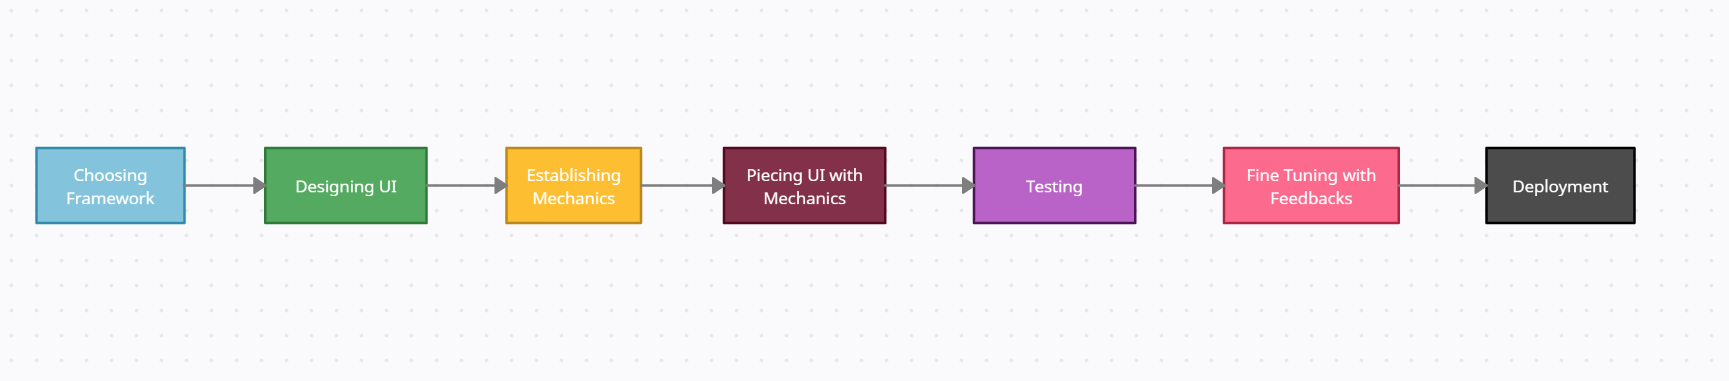
\includegraphics[scale=0.5]{SDLC.png}
\end{center}
\newpage

1.	Choosing Framework: The process of selecting a framework for our project was a crucial step, and we carefully evaluated different options before settling on Unity. We considered the ease of adoption, the quality of the documentation, and the level of community support for each engine.
2.	Designing UI: In terms of UI design, we were fortunate to have mentors with a keen sense of aesthetics who helped us create an interface that was both intuitive and visually appealing. We took great care to ensure that the UI complemented the gameplay mechanics and enhanced the user experience.

3.	Establishing Mechanics: Developing game mechanics that were accessible to players of all ages and skill levels was one of our primary goals. We spent a significant amount of time refining and simplifying the mechanics to ensure that they were easy to understand and provided a fun and engaging experience.

4.	Piecing UI with Mechanics: The mechanics were made in isolation and the UI designed differently since, we had to piece them together that really tells us the real story of development, fun and challenging at the same time. Integrating the UI and mechanics was a challenging but rewarding process. We designed them separately, which required us to carefully consider how they would work together and make the necessary adjustments to ensure that they were seamlessly integrated.

5.	Testing: Testing in gaming is a very strenuous job since there are many scopes to test with the available limited resources we have done Playtests, Network connection testing as well making sure there is no problem in mechanics and UI.Testing and quality assurance were critical components of our development process. We conducted extensive playtests, network connection testing, and comprehensive checks of mechanics and UI to ensure that the game was polished and free of bugs and glitches.

6.	Fine Tuning with Feedbacks: The edge and boundary cases of the game had a lot of bugs which led to backtracking our mistakes and making sure it was a tight ship. We encountered several bugs during the development process that required backtracking and debugging. We listened to feedback from players and continuously refined the game to ensure an optimal experience.

7.	Deployment: Deployment for a Unity cross platform has to be done across their own respective store so, for PC it is Steam or something for Apple their App Store and Android it is Google Play Store, since we are 4 students we chose to upload our game on itch.io for deployment and uploaded binaries for each platform, we chose itch.io since it is free and a lot of indie games are there already on it. Deploying a Unity cross-platform game requires uploading it to respective stores such as Steam for PC, Apple App Store for iOS, and Google Play Store for Android. As a team of four, we chose itch.io, a free platform that hosts many indie games, to upload our game. We uploaded binaries for each platform to itch.io.

\clearpage
%end of INtroduction

%start of Literature Survey
\centering
\section{LITERATURE SURVEY}
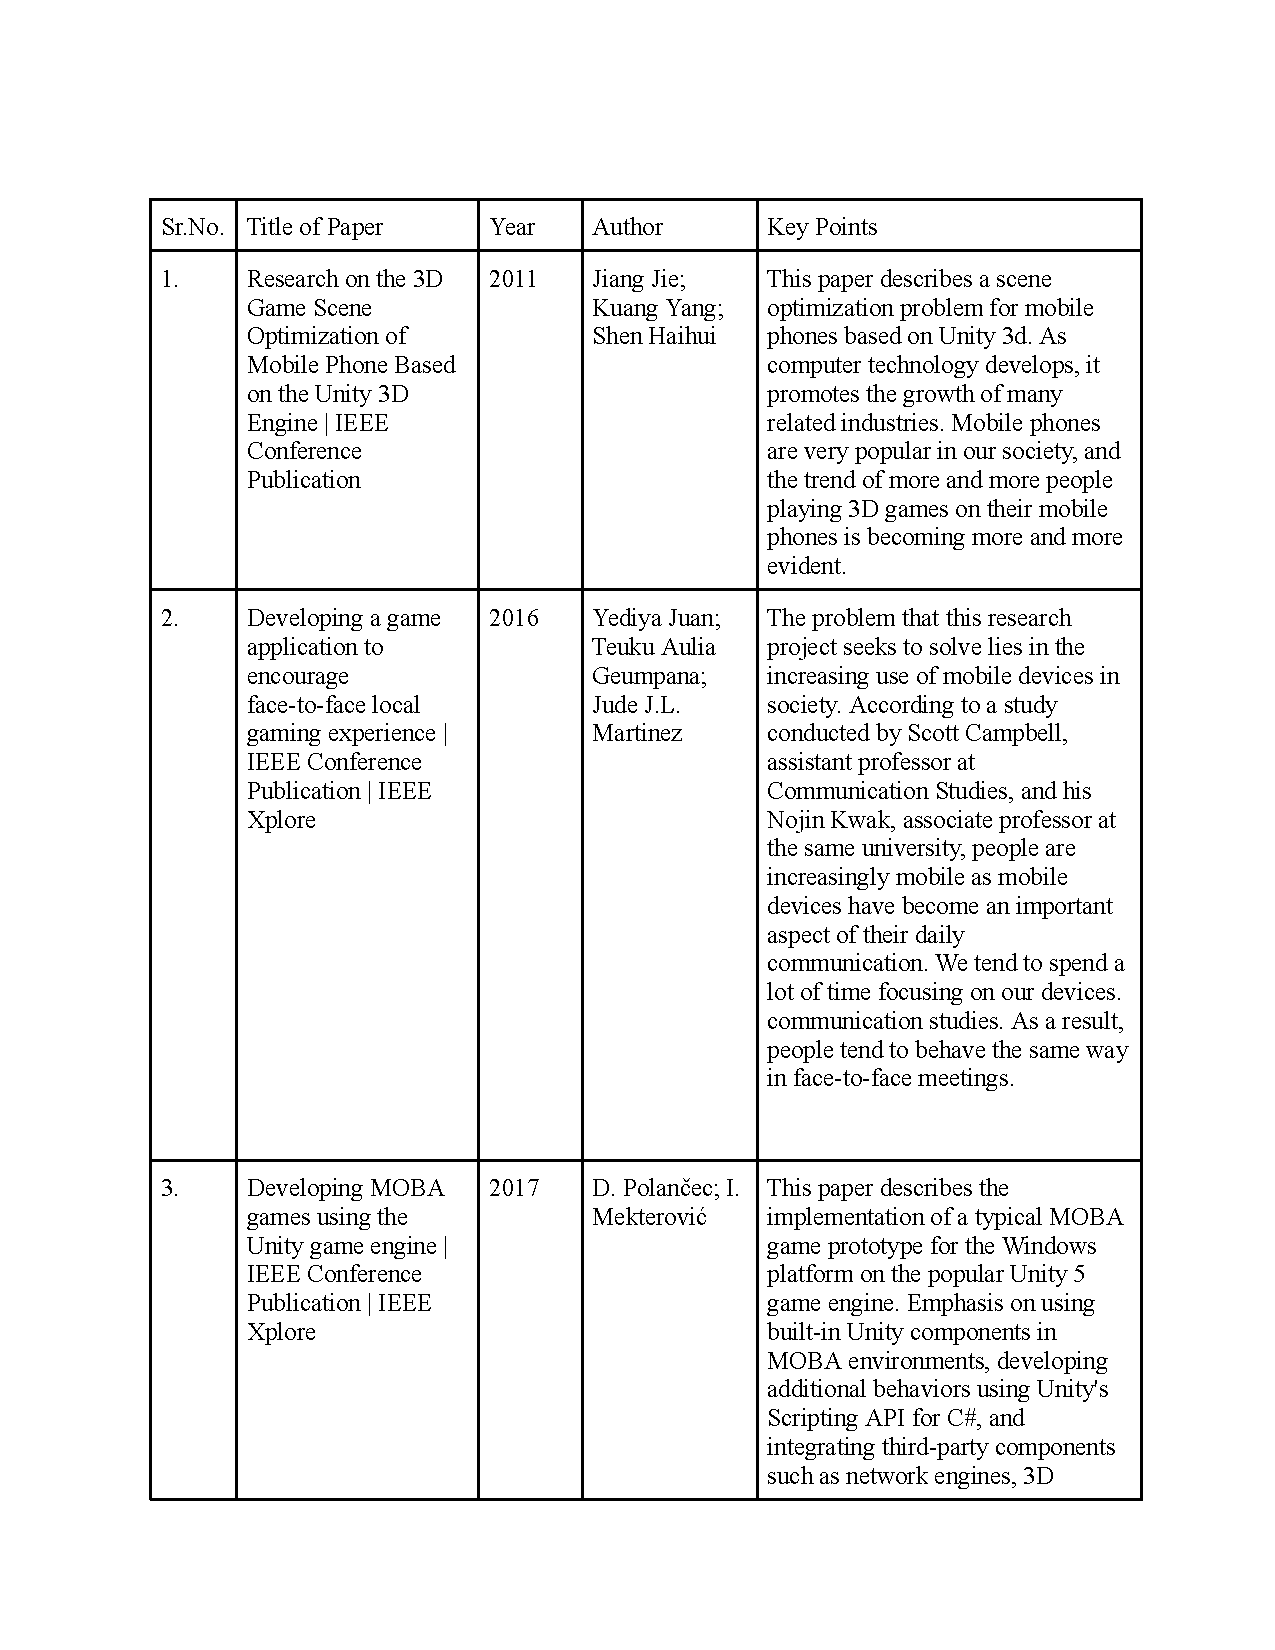
\includepdf[pages={1-} ,offset=0cm 0cm]{LitSurvey.pdf}
%end of litterature

% SOFTWARE REQUIREMENT SPECIFICATION
\centering
\section{SOFTWARE REQUIREMENT SPECIFICATION}
\raggedright
\subsection{Assumptions and Dependencies}

\justifying
\setlength{\parindent}{4em}
\setlength{\parskip}{0.5em}
\renewcommand{\baselinestretch}{1.5}

\normalsize
\hspace{1.7cm}\subsubsection{Assumptions:}
\begin{itemize}\item Players are familiar with the rules of dodgeball and understand the objective of the game.
\item Players have basic knowledge of gaming controls and mechanics.
\item Players have access to the necessary equipment, such as a computer or a gaming console, to play the game.
\item The game is designed for multiplayer mode, and players can connect to the game server without any issues.
\item The game mechanics are well-defined and allow players to perform all the necessary actions to play the game effectively.
\end{itemize}

% code to fig reffrence==[figure. \ref{Simple Cryptography Process}].
\hspace{1.7cm}\subsubsection{Dependencies:}
\begin{itemize}\item Players are familiar with the rules of dodgeball and understand the objective of the game.
\item The game depends on the underlying software infrastructure, such as the operating system, web server, and database server, to function correctly.
\item The game depends on network connectivity to connect players to the game server and enable multiplayer mode.
\item The game depends on the hardware capabilities of the player's device, such as the CPU, GPU, and RAM, to run smoothly and without any lag.
\item The game depends on the availability of game assets, such as graphics, sound effects, and music, to create a rich and immersive gaming experience.
\item The game's success depends on the availability of players to participate in multiplayer mode and engage with the game.
\end{itemize}

%\textbf{Domain}: Machine Learning\\
%\textbf{Input}: Users’ Face

\centering
\raggedright
\subsection{ FUNCTIONAL REQUIREMENT}

\justifying
\setlength{\parindent}{4em}
\setlength{\parskip}{0.5em}
\renewcommand{\baselinestretch}{1.5}

%\normalsize Proposed system consists of 4 modules:
\begin{itemize}\item After running the game, the UX view of the game will appear on the screen.
\item User Experience which is used to explain all aspects of a person's experience with a system.
\item The gamer can directly select "Start" from the "Main Menu"  which contains a number of Scenes like Tutorial, Matchmaking, Settings, and Quit.
\item During Tutorial and Matchmaking players can control the character and have features like pause and play and can change settings in mid-game.

\end{itemize}
\centering
\raggedright
\subsection{ EXTERNAL INTERFACE REQUIREMENT}

\justifying
\setlength{\parindent}{4em}
\setlength{\parskip}{0.5em}
\renewcommand{\baselinestretch}{1.5}
%\subsubsection{ User Interface}
\normalsize\begin{itemize}\item  Maximum high regulation with minimum hardware.
\item We may provide each player with their rank.
\item Easy to operate.
\item Minimum hardware requirements which are relevant for this game.
\item Design the whole system in an efficient manner.
\end{itemize}
\subsubsection{ User Interface}
%\normalsize\begin{itemize}\item   Hardware: Intel i5 Processor
%\item  Speed: 2.80 GHz
%\item  RAM: 8GB
%\item  Hard Disk: 64 GB
%\item  KeyBoard: Standard Windows Keyboard
%\end{itemize}
\subsubsection{ Hardware Interfaces:}
\normalsize

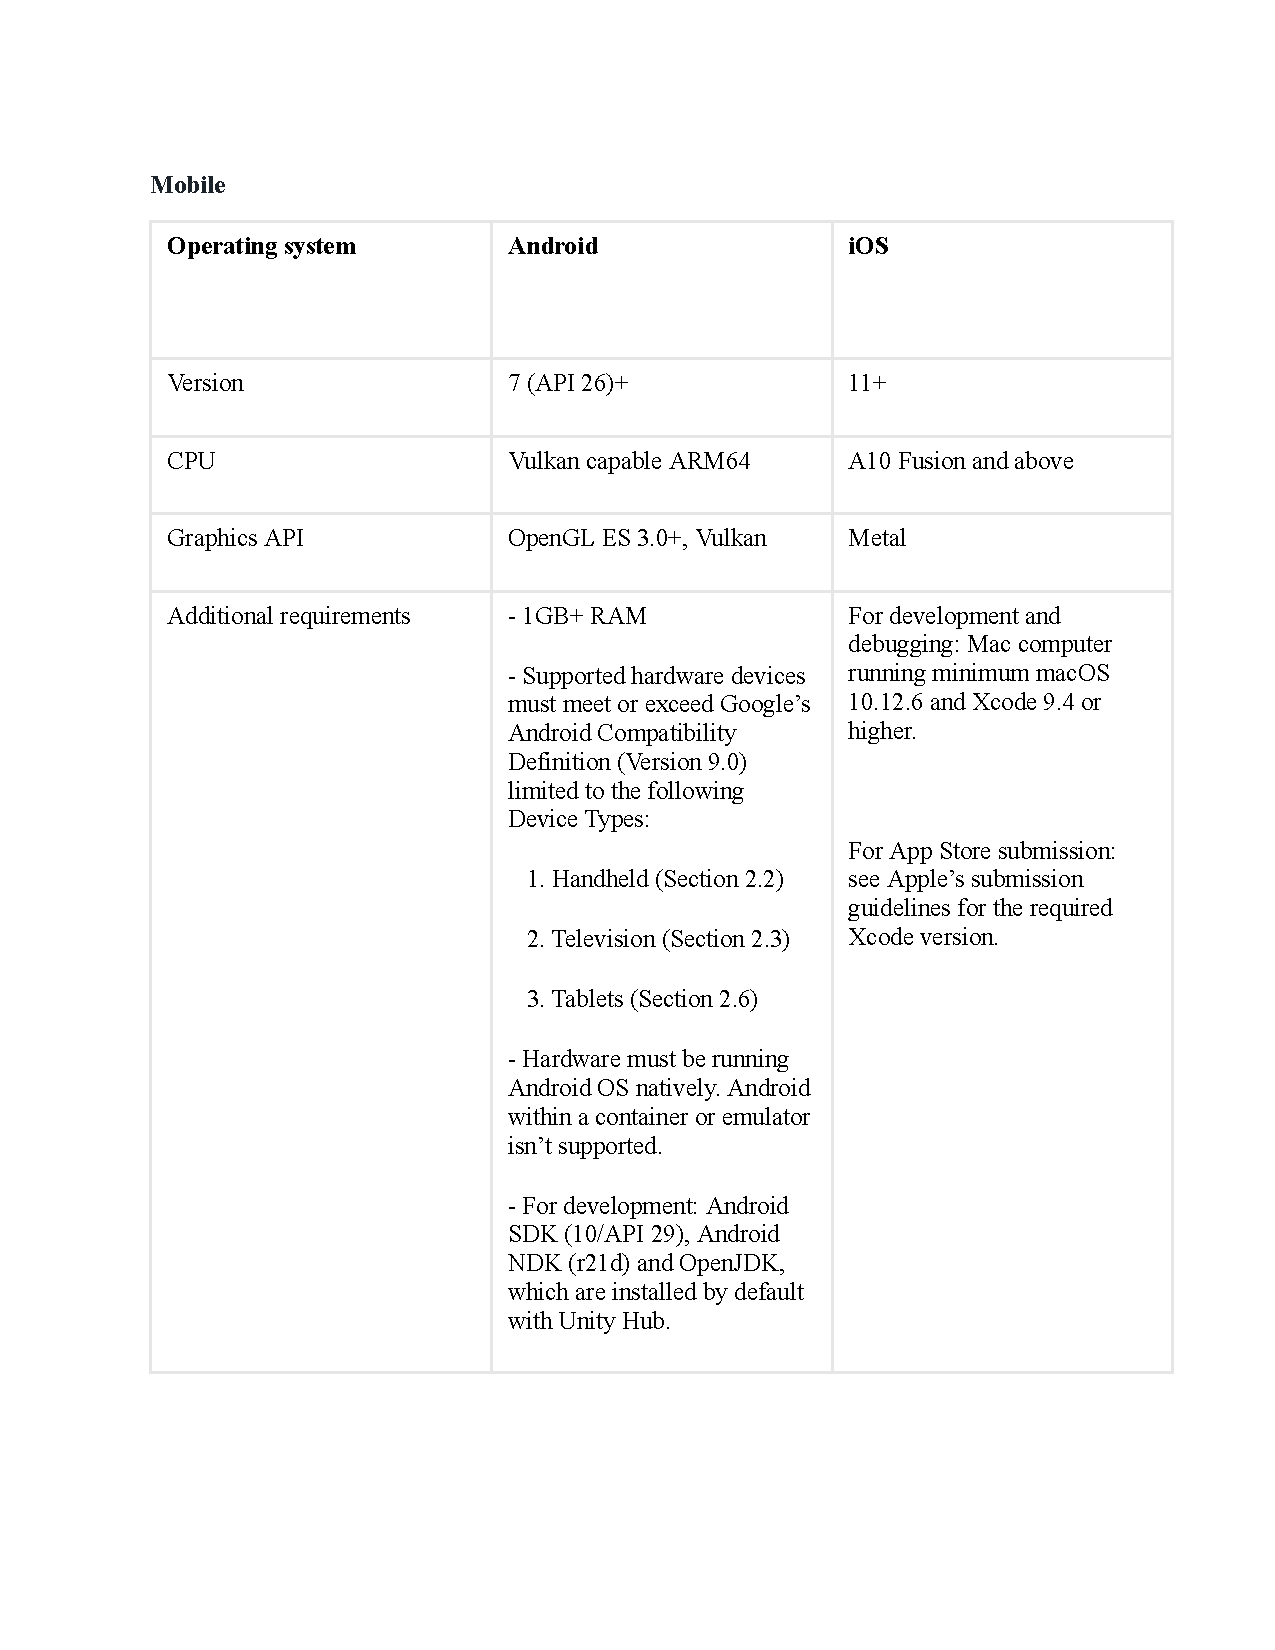
\includepdf[pages=-]{HardwareInfo.pdf}

\subsubsection{ Software Interfaces:}
\normalsize
\begin{itemize}
\item Operating System: Windows/macOS/Linux 

\item Game Engine: Unity 

\item Programming Language: C\#

\item Build Systems : .NET, Mono, Gradle, Xcode

\end{itemize}

\centering
\justifying
\setlength{\parindent}{0em}
\renewcommand{\baselinestretch}{1.5}
Unity: Unity is a cross-platform game engine developed by Unity Technologies, 
first announced and released in June 2005 at Apple Worldwide Developers Conference as a Mac OS X game engine.
The engine has since been gradually extended to support a variety of desktop, mobile, console, and virtual reality platforms.

\setlength{\parindent}{0em}
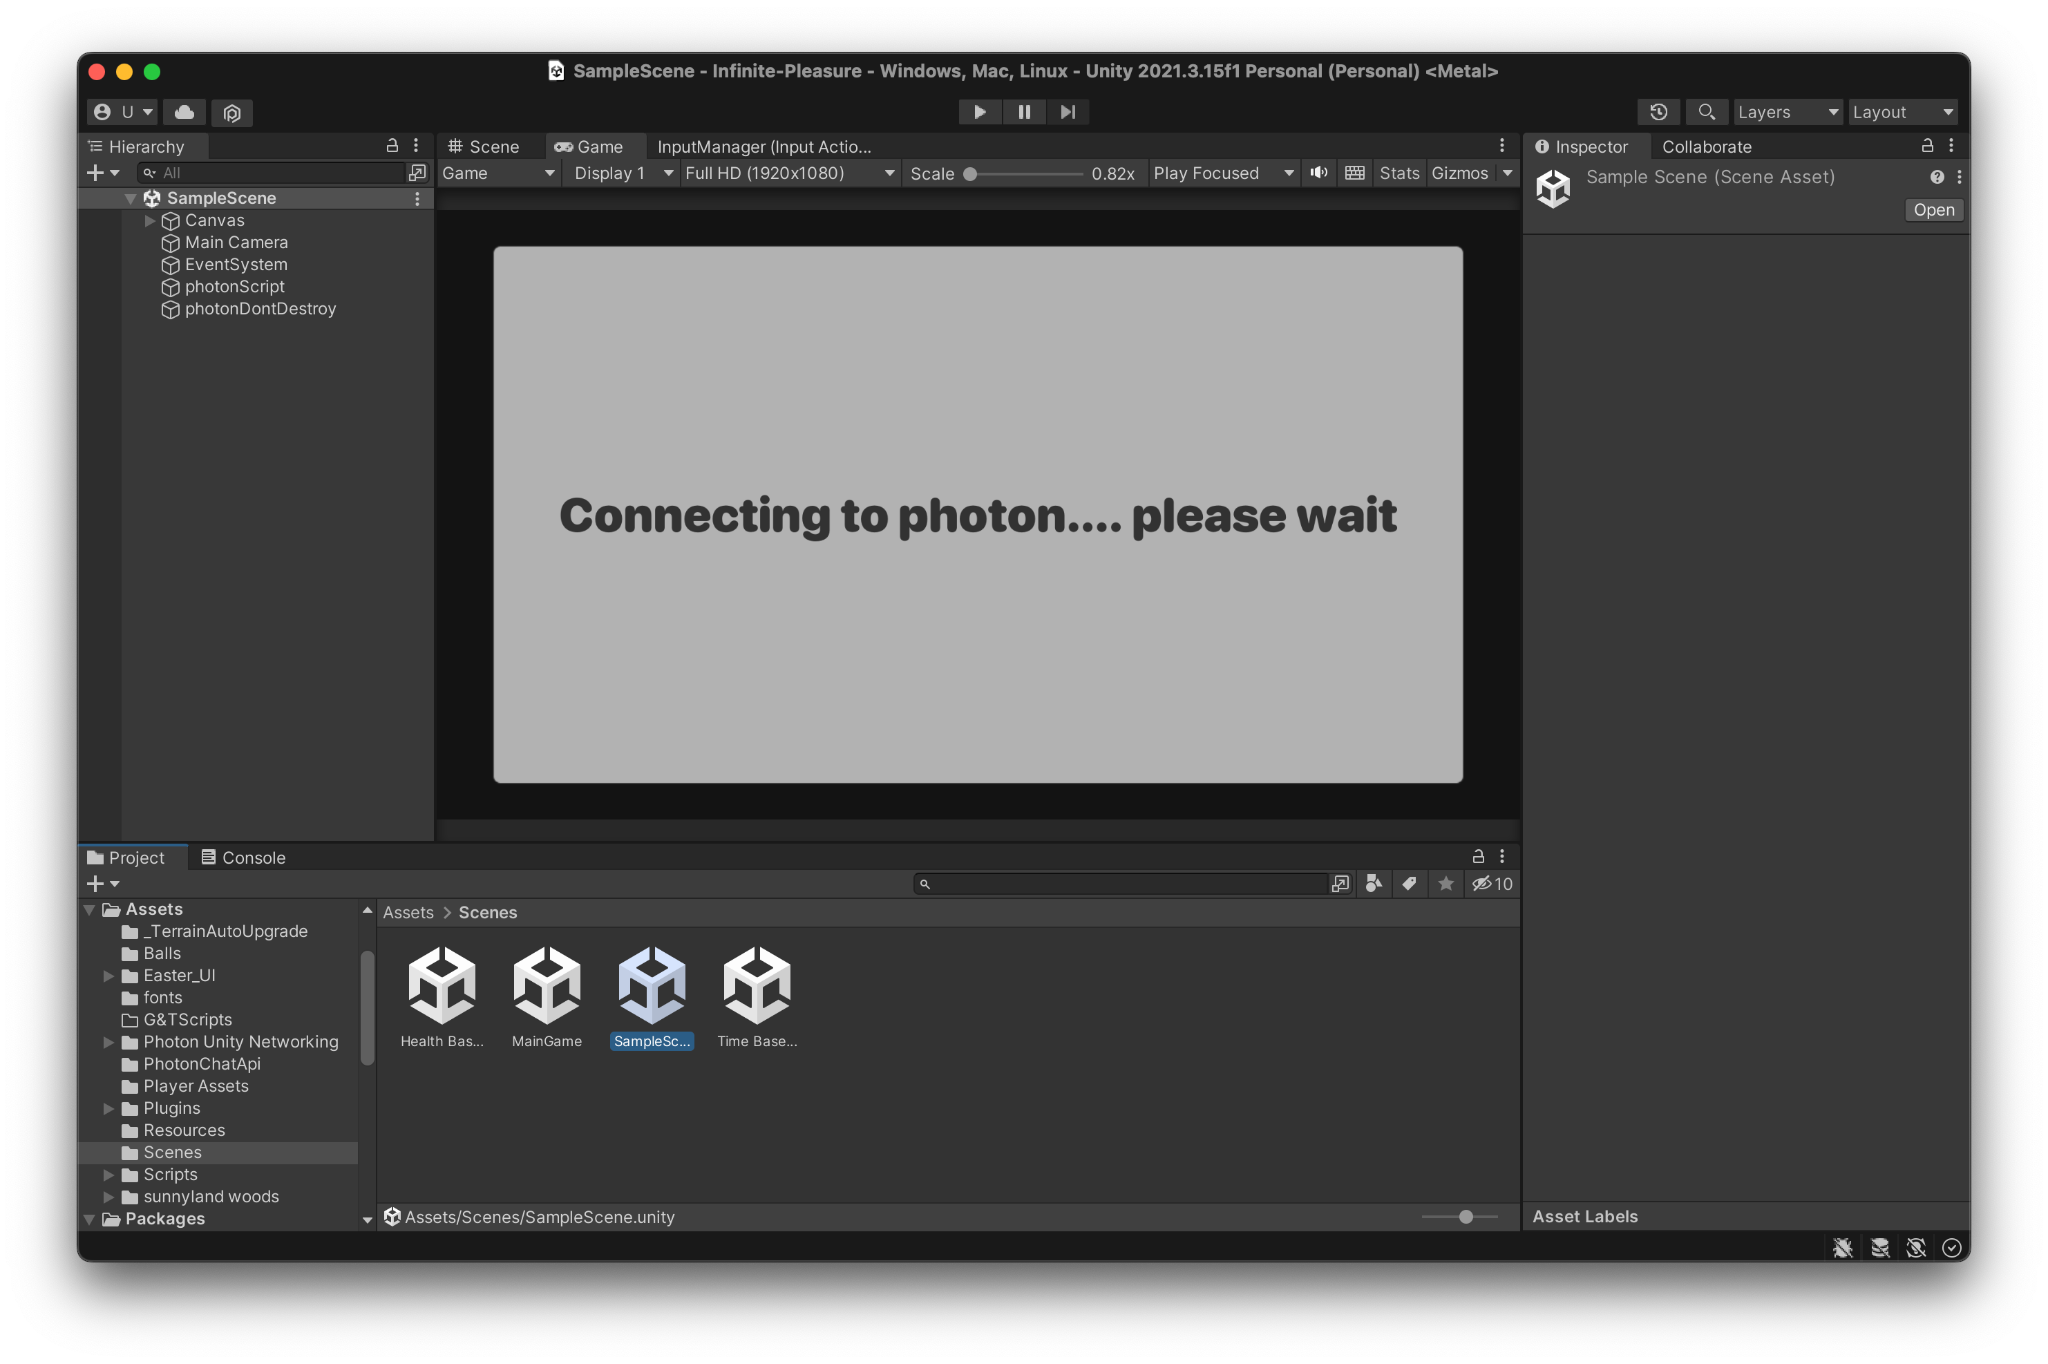
\includegraphics[scale=0.2]{Haar.png}

C-Sharp: C\# is a general-purpose, high-level multi-paradigm programming language. C\# encompasses static typing, strong typing, lexically scoped, imperative, declarative, functional, generic, object-oriented, and component-oriented programming disciplines. C-sharp (C\#) is a popular programming language developed by Microsoft in 2002. It has also been a main language for Unity game engine since 2005. Unity3D, being one of the two main obvious choices for AR/VR development, to get a handle of it if they want to develop applications with some complexity (think physics, animations, to design patterns, shaders or even sound effects).

Rider: JetBrains Rider is a fast and powerful C\# editor for Unity that runs on Windows, Mac, and Linux. With the unbeatable 2500+ smart code inspections and refactorings, Rider enhances your C\# experience, letting you write error-proof code much faster.

Visual Studio: is an integrated development environment from Microsoft.The Unity engine integrates into one unparalleled platform to create 2D and 3D games and interactive content. Create once and publish to 21 platforms, including all mobile platforms, WebGL, Mac, PC and Linux desktop, web or consoles. Visual Studio brings powerful features to C\# programmers. Write code quickly and with precision using IntelliSense. Navigate through your scripts easily and use powerful refactoring capabilities.

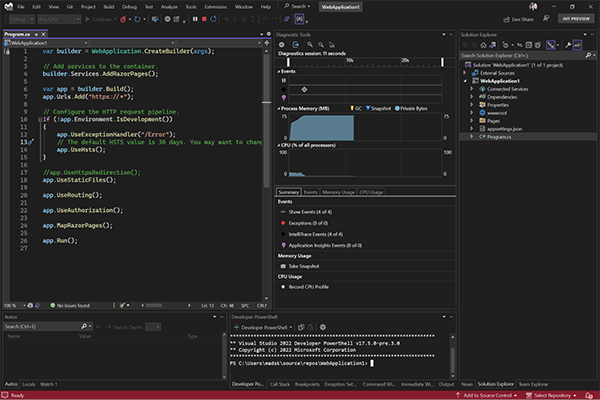
\includegraphics[scale=0.6]{image7.png}

Xcode: Xcode is Apple's integrated development environment for macOS, used to develop software for macOS, iOS, iPadOS, watchOS, and tvOS. It was initially released in late 2003; the latest stable release is version 14.1, released on November 1, 2022, via the Mac App Store with macOS Monterey. The new multi platform target creates a single interface for use across iOS, iPadOS, macOS, and tvOS. Your code is easier to maintain, and ready to be customized to take advantage of each platform’s unique capabilities.

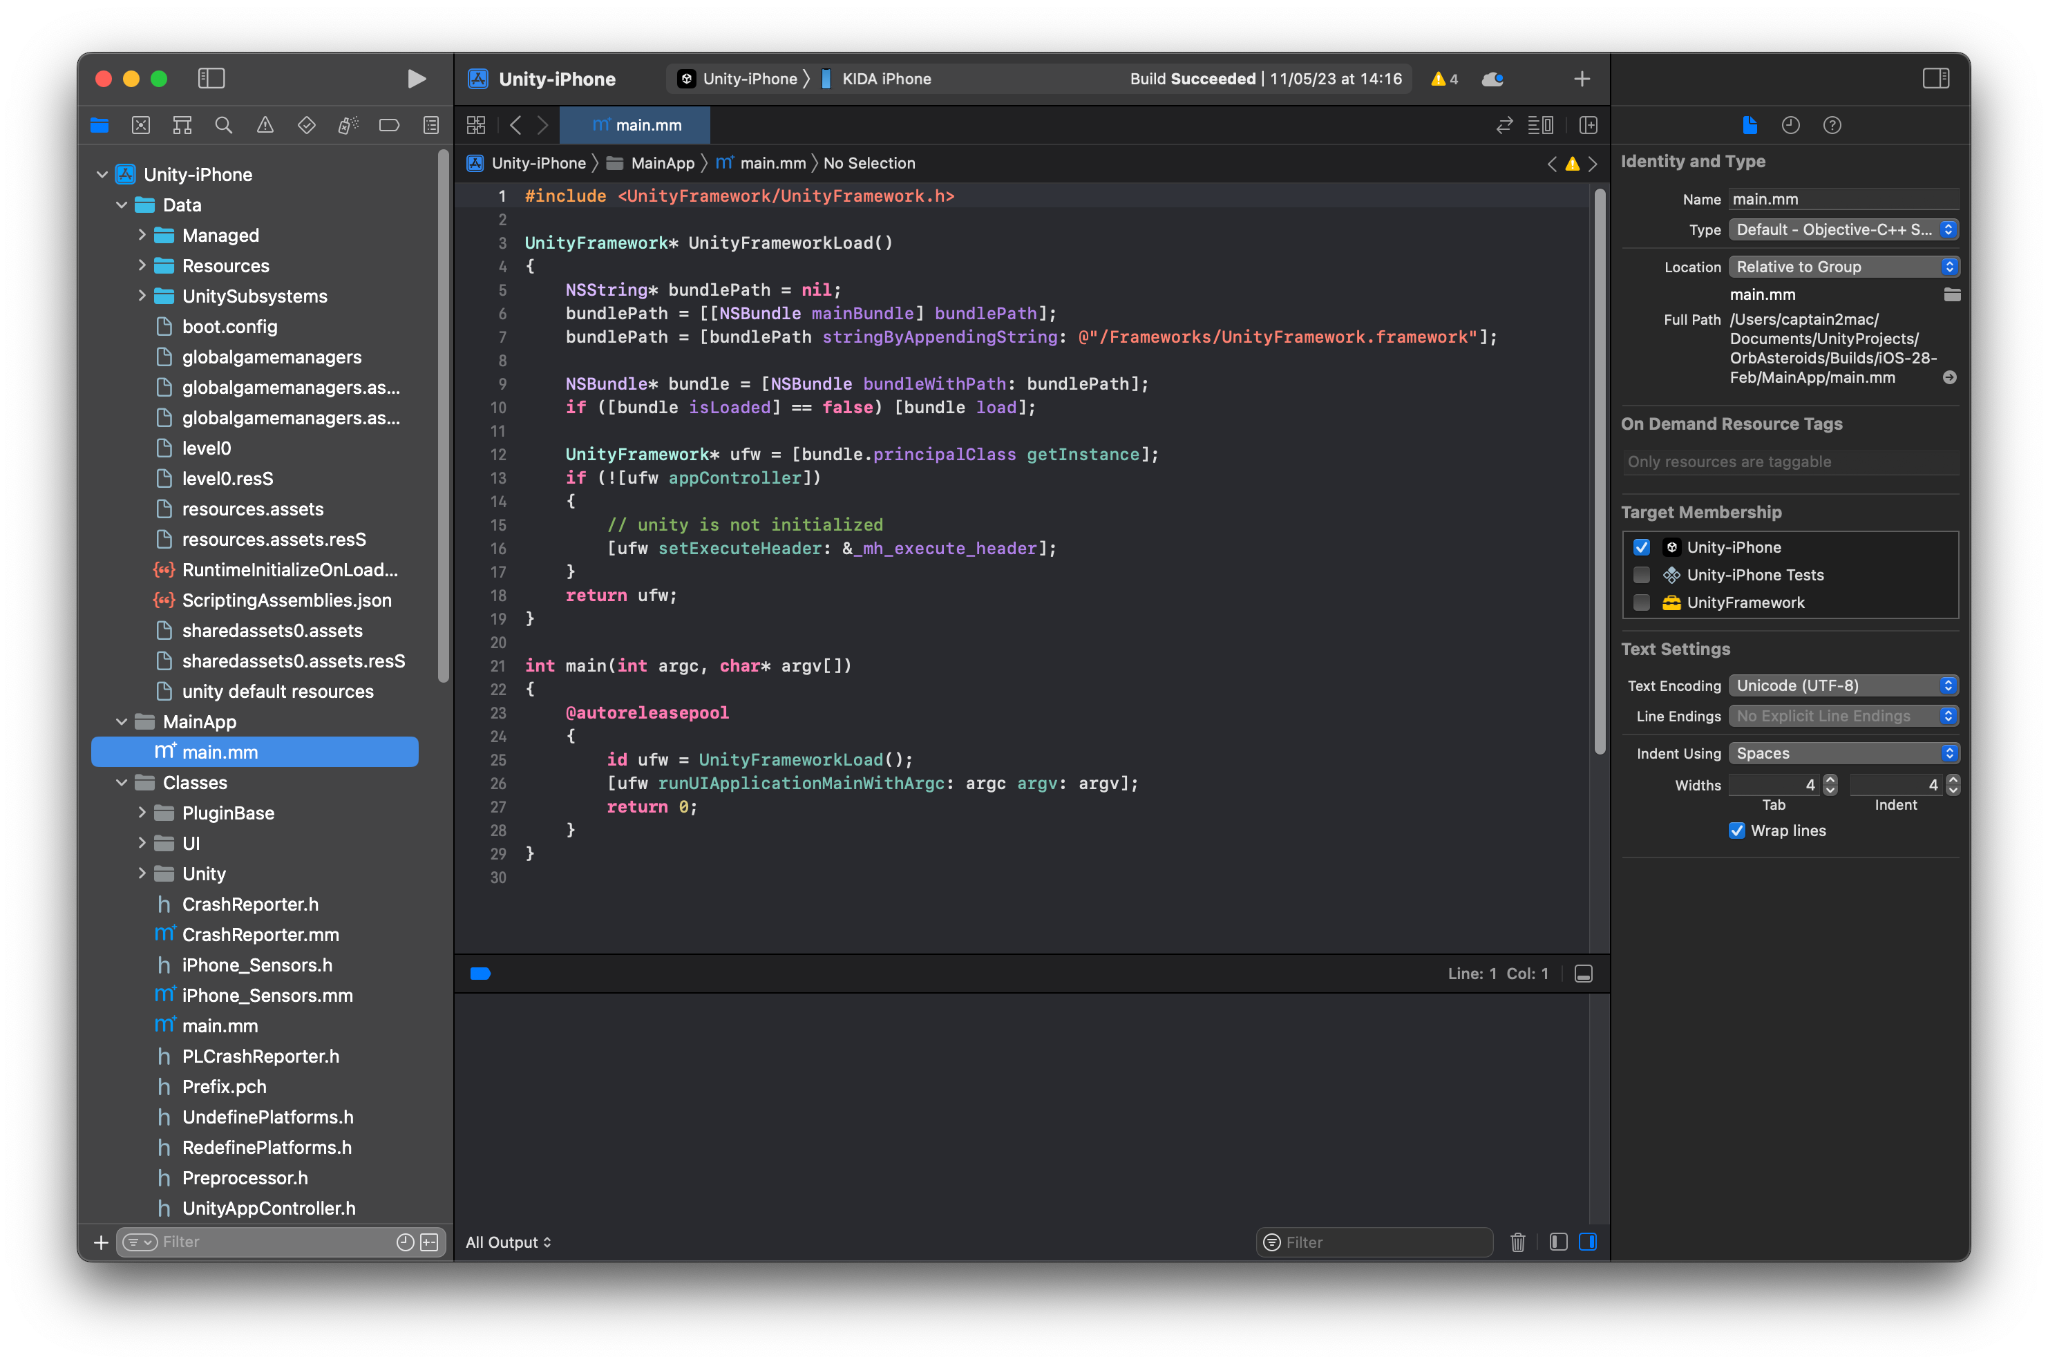
\includegraphics[scale=0.2]{image8.png}

Gradle: Gradle is a build automation tool for multi-language software development. It controls the development process in the tasks of compilation and packaging to testing, deployment, and publishing. Supported languages include Java, C/C++.

Mono: The Mono scripting backend compiles code at runtime, with a technique called just-in-time compilation (JIT). Unity uses a fork of the open source Mono project. Some platforms don’t support JIT compilation, so the Mono backend doesn’t work on every platform. Other platforms support JIT and Mono but not ahead-of-time compilation (AOT), and so can’t support the IL2CPP backend. When a platform can support both backends, Mono is the default.


\centering
\raggedright
\subsection{ NON-FUNCTIONAL REQUIREMENT}

\justifying
\setlength{\parindent}{4em}
\setlength{\parskip}{0.5em}
\renewcommand{\baselinestretch}{1.5}
\subsubsection{ Performance Requirements}
\normalsize\begin{itemize}
    \item The game will run on Android, MacOS, iOS, and Windows 10 (or newer) and requires the user to have the following components for Desktop: keyboard, mouse, monitor, and computer.
    \item The game will run with a CPU with SSE2 instruction set support and a Graphics card with DX10 (shader model 4.0) capabilities. Need a minimum of 4GB RAM, and 1GB of storage space.
    \item An Internet connection will also be required for multiplayer. The game will be running at a minimum of 1080p 60fps and a maximum of 1080p 120fps.
\end{itemize}

\subsubsection{ Safety Requirement}
\normalsize\begin{itemize}
    \item Age appropriateness: Clearly define the target audience for your game and ensure that the content, themes, and challenges are suitable for that age group. Implement age verification mechanisms if necessary.
    \item User privacy: Respect user privacy by implementing appropriate data protection measures. Clearly communicate your data collection and usage policies, and obtain user consent when necessary. Follow applicable data protection regulations, such as the General Data Protection Regulation (GDPR) if your game is available to users in the European Union.
    \item Online interactions: If your game includes online multiplayer features or chat functionality, implement measures to prevent and handle inappropriate behavior, harassment, and cyberbullying. Provide reporting and blocking mechanisms for users to address such issues.
    \item Parental controls: Consider implementing parental control features to allow parents or guardians to restrict access to certain content, set time limits, or manage in-game purchases for underage players.
    \item Game content warnings: Provide appropriate content warnings for potentially sensitive or disturbing content, such as violence, horror, or mature themes. Allow players to customize content filters if necessary.
    \item Accessibility: Ensure your game is accessible to players with disabilities. Implement features such as colorblind modes, adjustable font sizes, captioning for audio content, and support for alternative input devices.
    \item Fair gameplay: Prevent cheating, hacking, or exploiting in the game to maintain a fair and enjoyable experience for all players. Implement appropriate security measures and address any vulnerabilities promptly.
    \item Compliance with regulations: Familiarize yourself with applicable laws, regulations, and industry standards related to game safety, including consumer protection laws, advertising standards, and intellectual property rights.
    \item Apple IDFA: The Identifier for Advertisers (IDFA) is a random device identifier assigned by Apple to a user’s device. Advertisers use this to track data so they can deliver customized advertising. The IDFA is used for tracking and identifying a user (without revealing personal information).

\end{itemize}
\subsubsection{  Software Quality Attributes}

\normalsize
\begin{itemize}
    \item Usability: The game should be easy to navigate and play, with clear instructions and intuitive controls.
    \item Performance: The game should be responsive and run smoothly without any lag or glitches.
    \item Reliability: The game should function reliably and consistently without crashes or other technical issues.
    \item Maintainability: The game should be designed with maintainability in mind, with clear and well-organized code that is easy to update and modify.
    \item Security: The game should be secure, with measures in place to protect player data and prevent cheating.
    \item Scalability: The game should be able to handle a growing number of players and gameplay data without a significant decrease in performance.
    \item Compatibility: The game should be compatible with different devices, operating systems, and web browsers to reach a wider audience.
    \item Portability: The game should be easily portable between different platforms, such as mobile devices and desktop computers.
    \item Accessibility: The game should be designed to be accessible to players with different abilities, with features such as subtitles, audio descriptions, and color contrast options.
    By focusing on these software quality attributes, the 2D dodgeball game can provide a high-quality gameplay experience for players, increase engagement, and encourage repeat gameplay.
    
\end{itemize}

\centering
\raggedright
\subsection{ SYSTEM REQUIREMENTS}

\justifying
\setlength{\parindent}{4em}
\setlength{\parskip}{0.5em}
\renewcommand{\baselinestretch}{1.5}

\subsubsection{Software Requirements}

\normalsize

1. Operating System: Windows/macOS/Linux 

2. Game Engine: Unity 

3. Programming Language: C\#

Unity: Unity is a cross-platform game engine developed by Unity Technologies, first announced and released in June 2005 at Apple Worldwide Developers Conference as a Mac OS X game engine. The engine has since been gradually extended to support a variety of desktop, mobile, console, and virtual reality platforms.
The technology that we refer to as IL2CPP has two distinct parts.
An ahead-of-time (AOT) compiler
A runtime library to support the virtual machine
The AOT compiler translates Intermediate Language (IL), the low-level output from .NET compilers, to C++ source code. The runtime library provides services and abstractions like a garbage collector, platform-independent access to threads and files, and implementations of internal calls (native code which modifies managed data structures directly).
The IL2CPP AOT compiler is named il2cpp.exe. On Windows you can find it in the Editor\\Data\\il2cpp directory. On OSX it is in the Contents/Frameworks/il2cpp/build directory in the Unity installation. The il2cpp.exe utility is a managed executable, written entirely in C\#. We compile it with both .NET and Mono compilers during our development of IL2CPP.
The il2cpp.exe utility accepts managed assemblies compiled with the Mono compiler that ships with Unity and generates C++ code which we pass on to a platform-specific C++ compiler.

\subsubsection{Hardware Requirements}
\hspace{1.7cm}
The hardware requirements for a Unity dodgeball game will depend on the complexity of the game, the graphics and physics involved, and the target platform (e.g., PC, mobile, console). Here are some considerations when determining the hardware requirements:

Processor (CPU): Unity games typically rely on the CPU for gameplay and physics calculations. A multi-core processor with a higher clock speed will help handle complex calculations more efficiently.

Graphics Card (GPU): The GPU handles rendering and graphics-related tasks. A dedicated graphics card with decent performance will ensure smooth rendering and better visual quality. The specific requirements will depend on the level of graphics fidelity desired for the game.
Here are the specific requirements for different platforms:

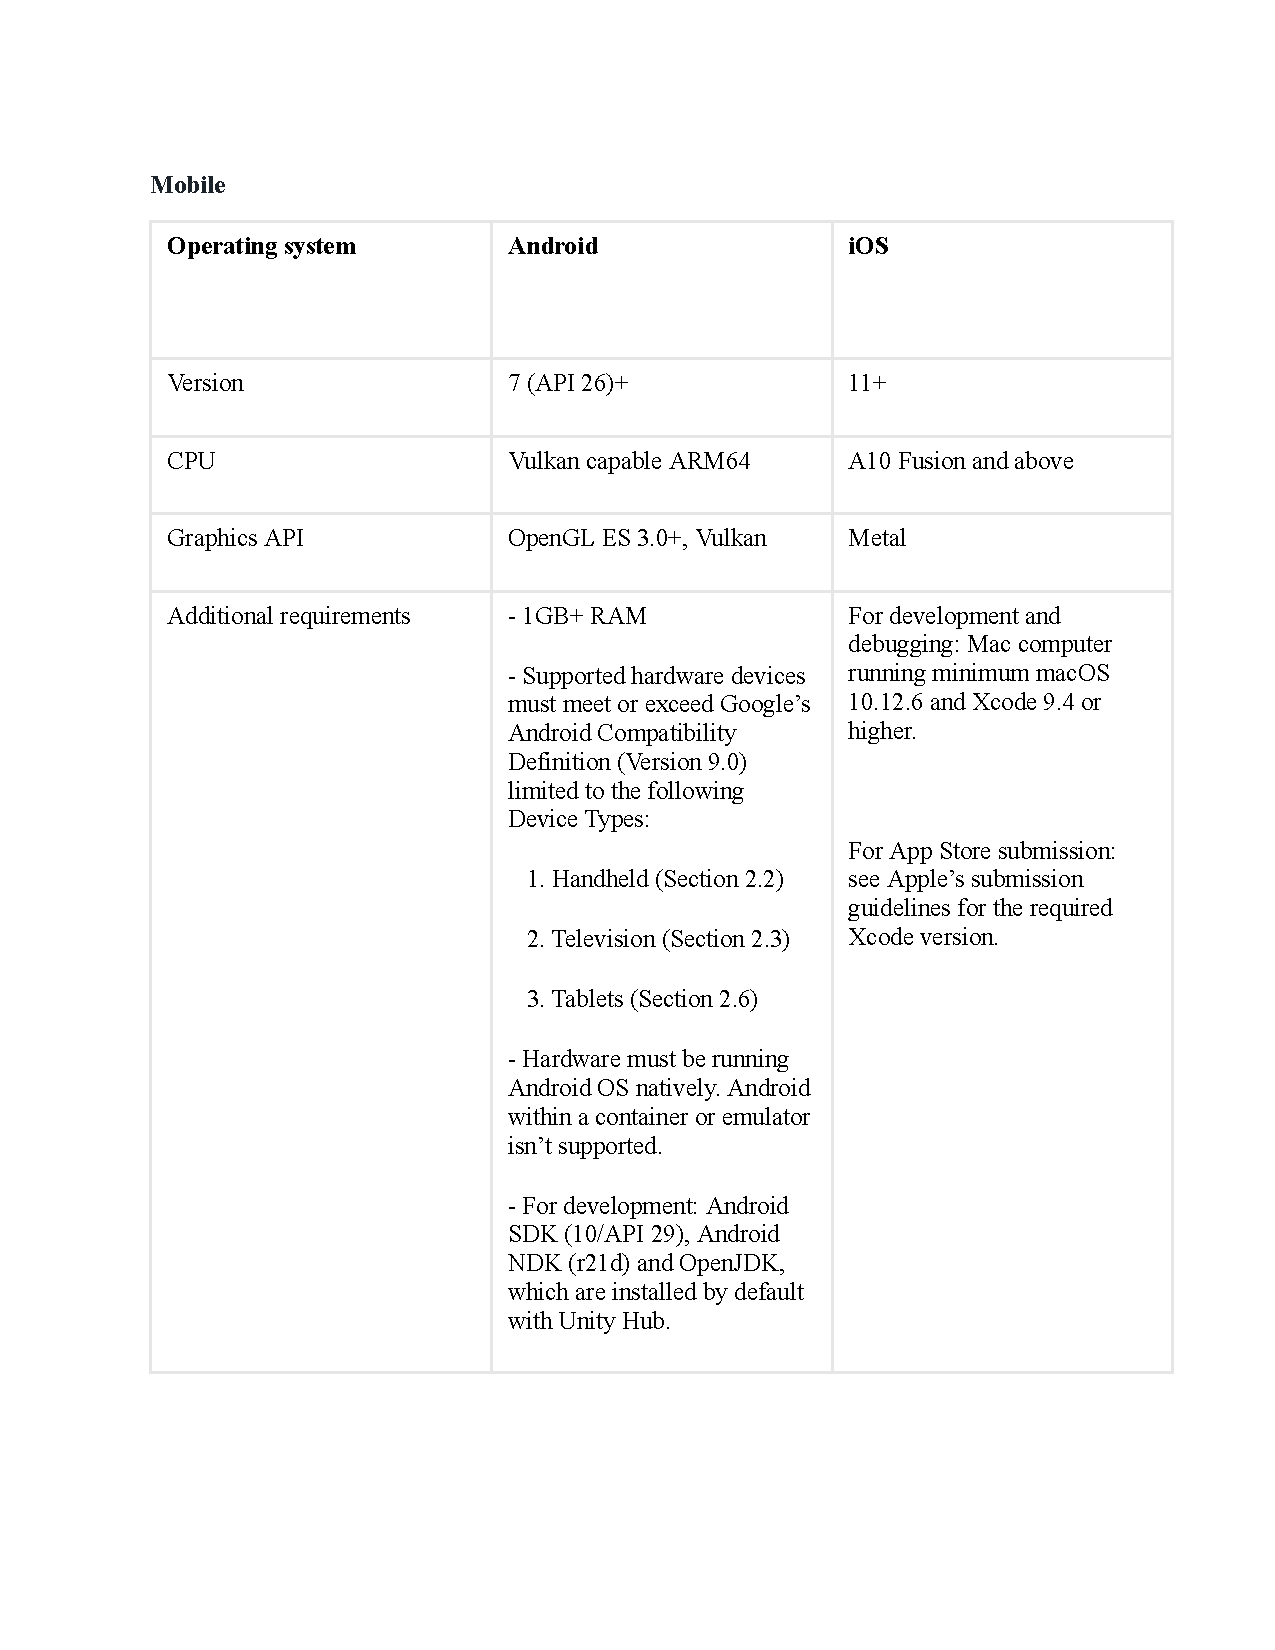
\includepdf[pages=-]{HardwareInfo.pdf}

\centering
\raggedright
\subsection{  ANALYSIS MODELS: SDLC MODEL TO BE APPLIED}

\justifying
\setlength{\parindent}{4em}
\setlength{\parskip}{0.5em}
\renewcommand{\baselinestretch}{1.5}
% \subsubsection{ User Interface}

\vspace{2cm}
\begin{figure}[h]
\centering
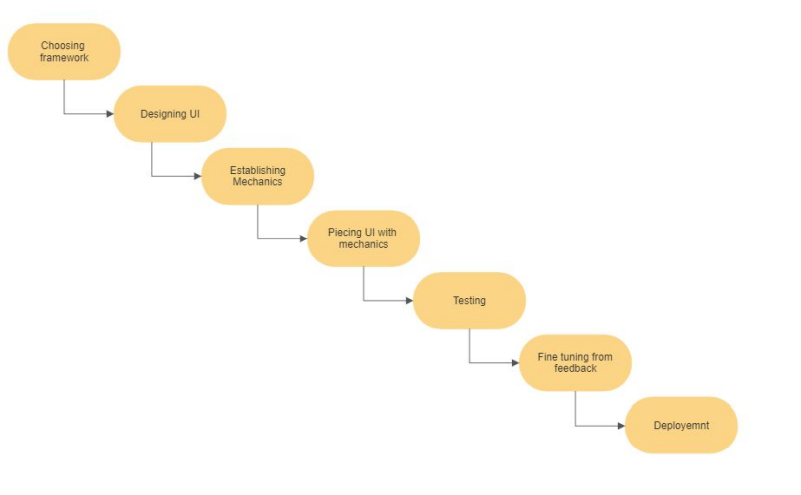
\includegraphics[scale=0.9]{Class Diagram.png}
\caption{SDLC MODEL}
\label{SDLC}
\end{figure}

\normalsize
SDLC Models stands for Software Development Life Cycle Models.
There are several software development life cycle (SDLC) models that can be applied in game development.
Let's take a look at a few examples:

Waterfall Model: The Waterfall Model is a linear sequential approach that involves a series of sequential phases. This model can be applied in game development by breaking down the game development process into different stages such as planning, design, implementation, testing, and maintenance. Each stage is completed before moving on to the next stage, and changes to previous stages are not allowed. This model is useful when the game requirements are well-defined and the project scope is clear.

Agile Model: The Agile Model is an iterative and incremental approach that involves continuous development and testing. This model can be applied in game development by breaking down the game development process into short development cycles called sprints. Each sprint involves designing, developing, testing, and integrating a small part of the game. The game is then tested and evaluated after each sprint, and changes are made accordingly. This model is useful when the game requirements are not well-defined, or when the project scope is subject to change.

Spiral Model: The Spiral Model is a risk-driven model that involves identifying and mitigating risks at each stage of the development process. This model can be applied in game development by breaking down the game development process into different stages, each involving risk analysis and mitigation. The game is then developed and tested, and the risks are reevaluated and mitigated in subsequent stages. This model is useful when the game requirements are not well-defined, or when the project scope is subject to change.

V-Model: The V-Model is a variation of the Waterfall Model that involves testing at each stage of the development process. This model can be applied in game development by breaking down the game development process into different stages, each involving testing and verification. The game is then developed and tested, and the testing results are used to verify and validate the game requirements. This model is useful when the game requirements are well-defined and the project scope is clear, but the testing and verification process is crucial.

Ours is:
Planning: During the planning phase, the team identifies the objectives and requirements for the game. They define the game mechanics, art style, target audience, and development timeline.

Analysis: In the analysis phase, the team evaluates the feasibility of the project and identifies potential risks. They analyze the game mechanics, UI design, and overall user experience to ensure that they meet the requirements set during the planning phase.

Design: During the design phase, the team creates detailed design documents that outline the game mechanics, level designs, and UI layout. They create wireframes, storyboards, and mockups to visualize the game design.

Development: In the development phase, the team begins coding the game using Unity. They implement the game mechanics, UI, and art assets created during the design phase. The team also conducts regular testing to identify and fix any bugs that may arise.

Testing: In the testing phase, the team conducts comprehensive testing to ensure that the game is stable, functional, and meets the user requirements. They conduct unit testing, integration testing, and acceptance testing to ensure the game is ready for release.

Deployment: During the deployment phase, the team releases the game to the appropriate platforms such as itch.io or other app stores. They ensure that the game meets the platform requirements and fix any issues that may arise during deployment.

Maintenance: After the game is released, the team continues to monitor and maintain the game to ensure it remains stable, secure, and enjoyable for players. They may release patches and updates to address bugs, improve gameplay, and add new features based on user feedback.


\clearpage
% end of SRS

%  SYSTEM DESIGN

\centering
\section{ SYSTEM DESIGN}
\raggedright
\subsection{SYSTEM ARCHITECTURE}

\justifying
\setlength{\parindent}{4em}
\setlength{\parskip}{0.5em}
\renewcommand{\baselinestretch}{1.5}

\vspace{0.5cm}
\begin{figure}[h]
\centering
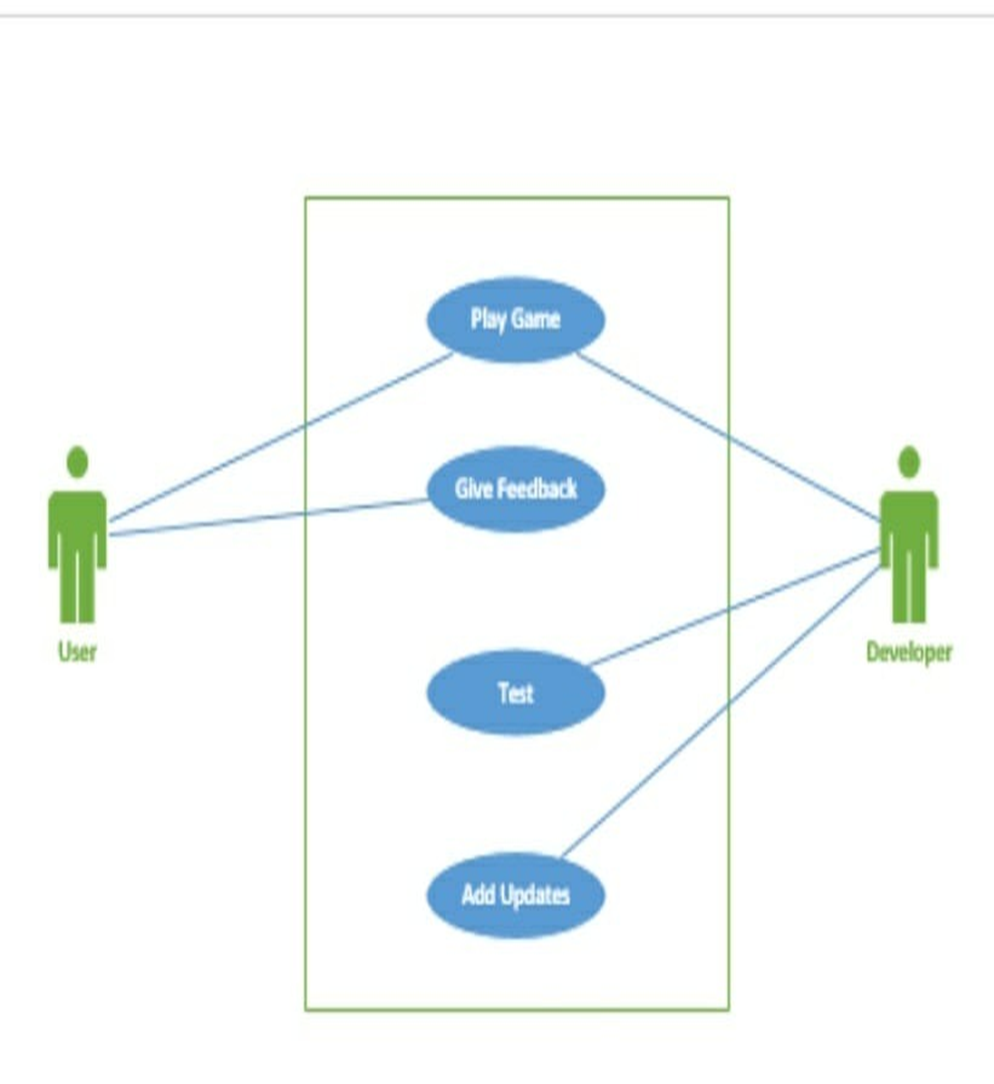
\includegraphics[scale=0.7]{Architecture.png}
\caption{ System Architecture}
\label{ System Architecture}
\end{figure}
\vspace{0.1cm}


\large\textbf{MATHEMATIC MODEL}
\normalsize
\justifying
\setlength{\parindent}{4em}
\setlength{\parskip}{0.5em}
\renewcommand{\baselinestretch}{1.5}
\vspace{0.1cm}
\begin{enumerate}
\item Player positions:
Let P1(x1, y1) and P2(x2, y2) represent the positions of Player 1 and Player 2 on a 2D plane.

\item Position and Velocity:
Let B(x, y) represent the position of the ball on the 2D plane.
Let Vx and Vy represent the ball's velocity components in the x and y directions.

\item Player movement:
Players can move in the x and y directions. Let $\Delta\mathrm{R}$x1, $\Delta\mathrm{R}$y1, $\Delta\mathrm{R}$x2, and $\Delta\mathrm{R}$y2 represent the changes in position for Player 1 and Player 2, respectively.
P1\_new(x1 + $\Delta\mathrm{R}$x1, y1 + $\Delta\mathrm{R}$y1) and P2\_new(x2 + $\Delta\mathrm{R}$x2, y2 + $\Delta\mathrm{R}$y2) represent the new positions of Player 1 and Player 2 after movement.

\item Ball movement:
The ball's position changes based on its velocity: B\_new(x + Vx * t, y + Vy * t), where t is the time elapsed since the last position update.

\item Throwing the ball:
When a player throws the ball, the ball's velocity components (Vx, Vy) are updated based on the throw's direction and strength.

\item Collision detection:
To determine if the ball hits a player, calculate the distance between the ball and each player using the Euclidean distance formula: d = sqrt((x2 - x1)\^2 + (y2 - y1)\^2).
If the distance is less than or equal to a predefined threshold (e.g., the sum of the player's and ball's radii), the player is considered hit.

\item Scoring and game state:
When a player is hit, the opposing player scores a point.
The game continues until a predefined number of points are scored by one of the players, or a time limit is reached.


\end{enumerate}
%end of design


\clearpage

\vspace{4cm}
\raggedright
\centering
\section{DIAGRAMS}
\justifying
\setlength{\parindent}{4em}
\setlength{\parskip}{0.5em}
\renewcommand{\baselinestretch}{1.5}
\normalsize
\subsection{Data Flow Diagram}
In Data Flow Diagram, we Show that flow of data in our system in DFD0 we show that 
base DFD in which rectangle present input as well as output and circle show our system. 
In DFD1 we show actual input and actual output of system input of our system is text or 
image and output is rumor detected likewise in DFD 2 we presentoperation of user as well
as admin.

\vspace{1cm}
\begin{figure}[h]
\centering
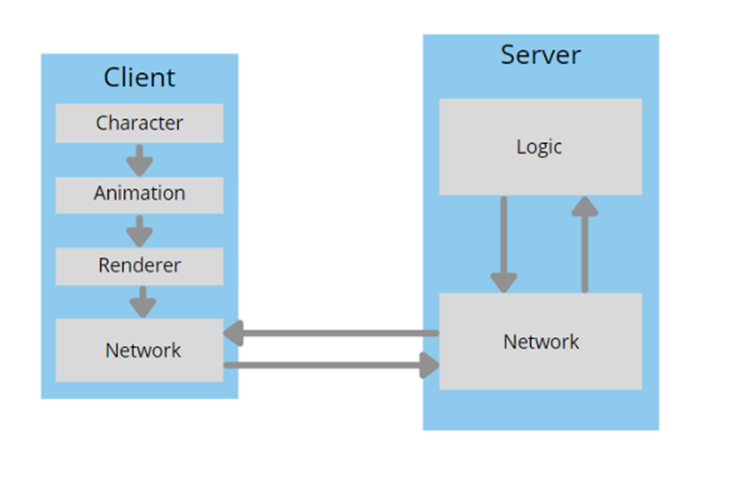
\includegraphics[scale=0.7]{ Data Flow diagram-0.png}
\caption{ Data Flow diagram-0}
\label{ Data Flow diagram-0}
\end{figure}


\vspace{1cm}
\begin{figure}[h]
\centering
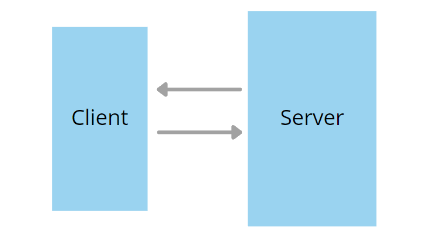
\includegraphics[scale=0.8]{ Data Flow diagram-1.png}
\caption{ Data Flow diagram-1}
\label{ Data Flow diagram-1}
\end{figure}



\vspace{1.5cm}
\begin{figure}[h]
\centering
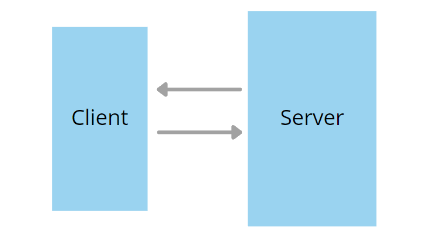
\includegraphics[scale=1.0]{ Data Flow diagram-1.png}
\caption{ Data Flow diagram-2}
\label{ Data Flow diagram-2}
\end{figure}


\clearpage
\justifying
\setlength{\parindent}{4em}
\setlength{\parskip}{0.5em}
\renewcommand{\baselinestretch}{1.5}
\normalsize
\subsection{UML DIAGRAMS}
Unified Modeling Language is a standard language for writing software blueprints. The
UML may be used to visualize, specify, construct and document the artifacts of a soft- ware
intensive system. UML is process independent, although optimally it should be used in
process that is use case driven, architecture centric, iterative and incremental. The Number
of UML Diagram is available.


\begin{itemize}
\item Use case Diagram.

\item Component Diagram.

\item Activity Diagram

\item  Sequence Diagram.

\end{itemize}

\clearpage


\justifying
\setlength{\parindent}{4em}
\setlength{\parskip}{0.5em}
\renewcommand{\baselinestretch}{1.5}
\normalsize
\subsection{Use Case Diagram}
A use case diagram in the Unified Modelling Language (UML) is a type of behavioral
diagram defined by and created from a Use-case analysis. Its purpose is to present a graphical 
overview of the functionality provided by a system in terms of actors, their goals 
(represented as use cases), and any dependencies between those use cases. The main purpose 
of a use case diagram is to show what system functions are performed for which actor. Roles 
of the actors in the system can be depicted.


\vspace{1.5cm}
\begin{figure}[h]
\centering
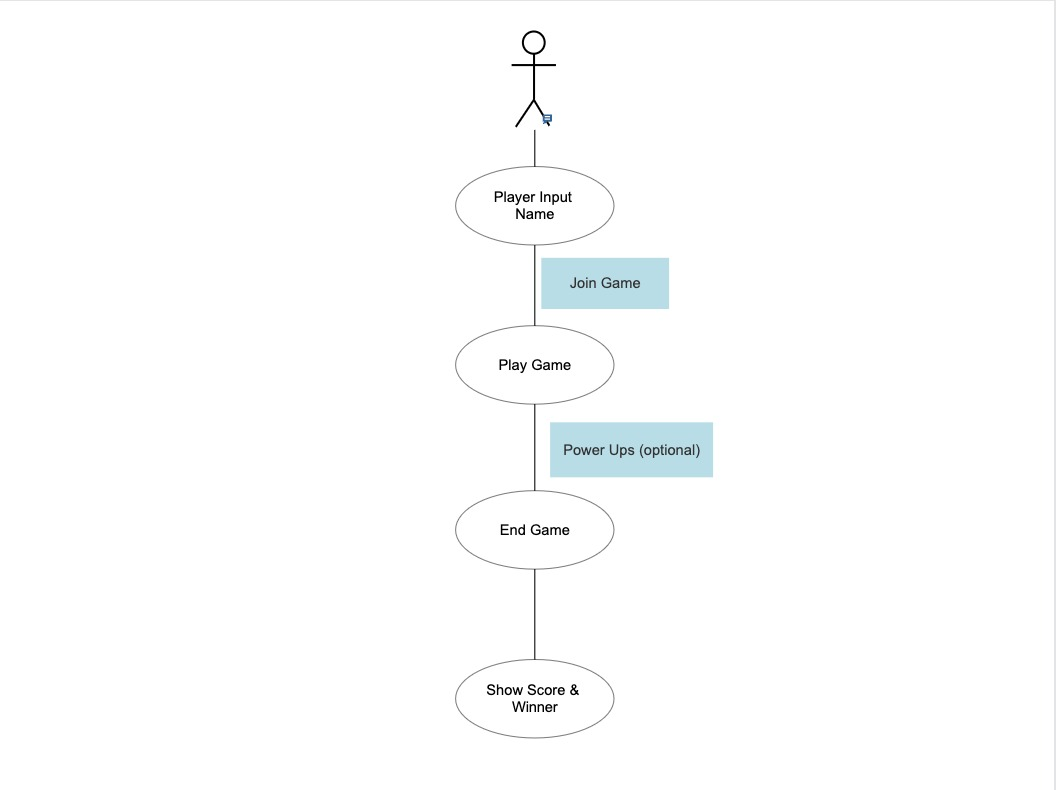
\includegraphics[scale=0.7]{images15.png}
\caption{Use case Diagram}
\label{ Use case Diagram}
\end{figure}

\justifying
\setlength{\parindent}{4em}
\setlength{\parskip}{0.5em}
\renewcommand{\baselinestretch}{1.5}
\normalsize
\subsection{Activity Diagram}
An activity is particular operation of the system. An activity diagram is intended to represent
stepwise work-flow of activities or actions that can take place in the system. It shows overall
flow of control and models computational and organizational processes. Activity diagrams
are used to model dynamic aspects of the system. 

\vspace{1.5cm}
\begin{figure}[h]
\centering
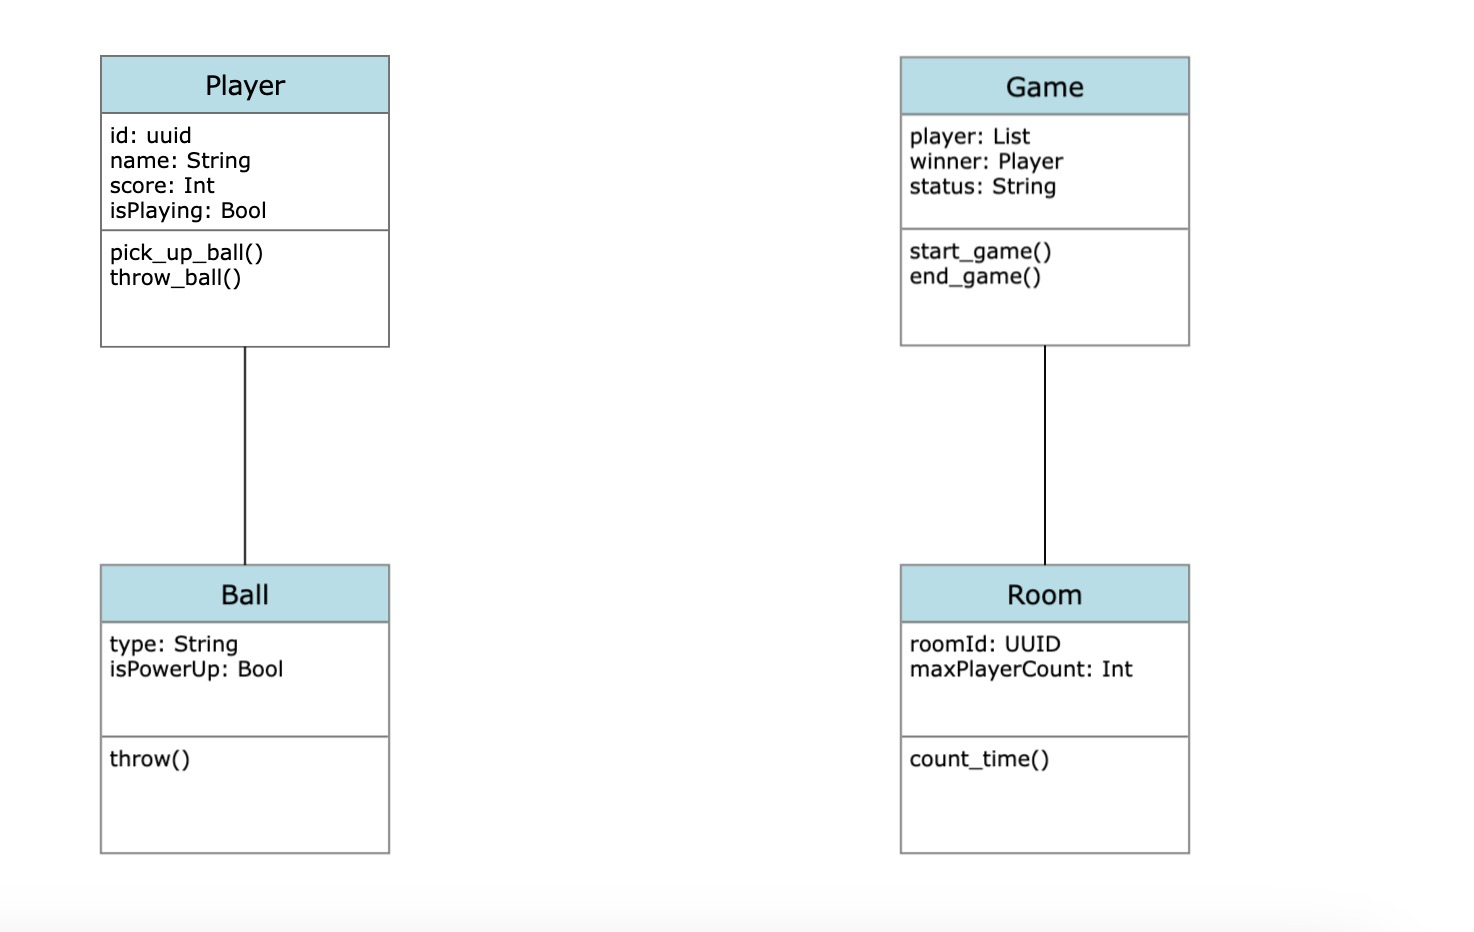
\includegraphics[scale=0.8]{images14.png}
\caption{Activity Diagram}
\label{Activity Diagram}
\end{figure}


\justifying
\setlength{\parindent}{4em}
\setlength{\parskip}{0.5em}
\renewcommand{\baselinestretch}{1.5}
\normalsize
\subsection{Sequence Diagram}
Sequence diagram shows how objects communicate with each other in terms of a sequence 
of messages. It also indicates the lifespans of objects relative to those messages.
\vspace{1.5cm}
\begin{figure}[h]
\centering
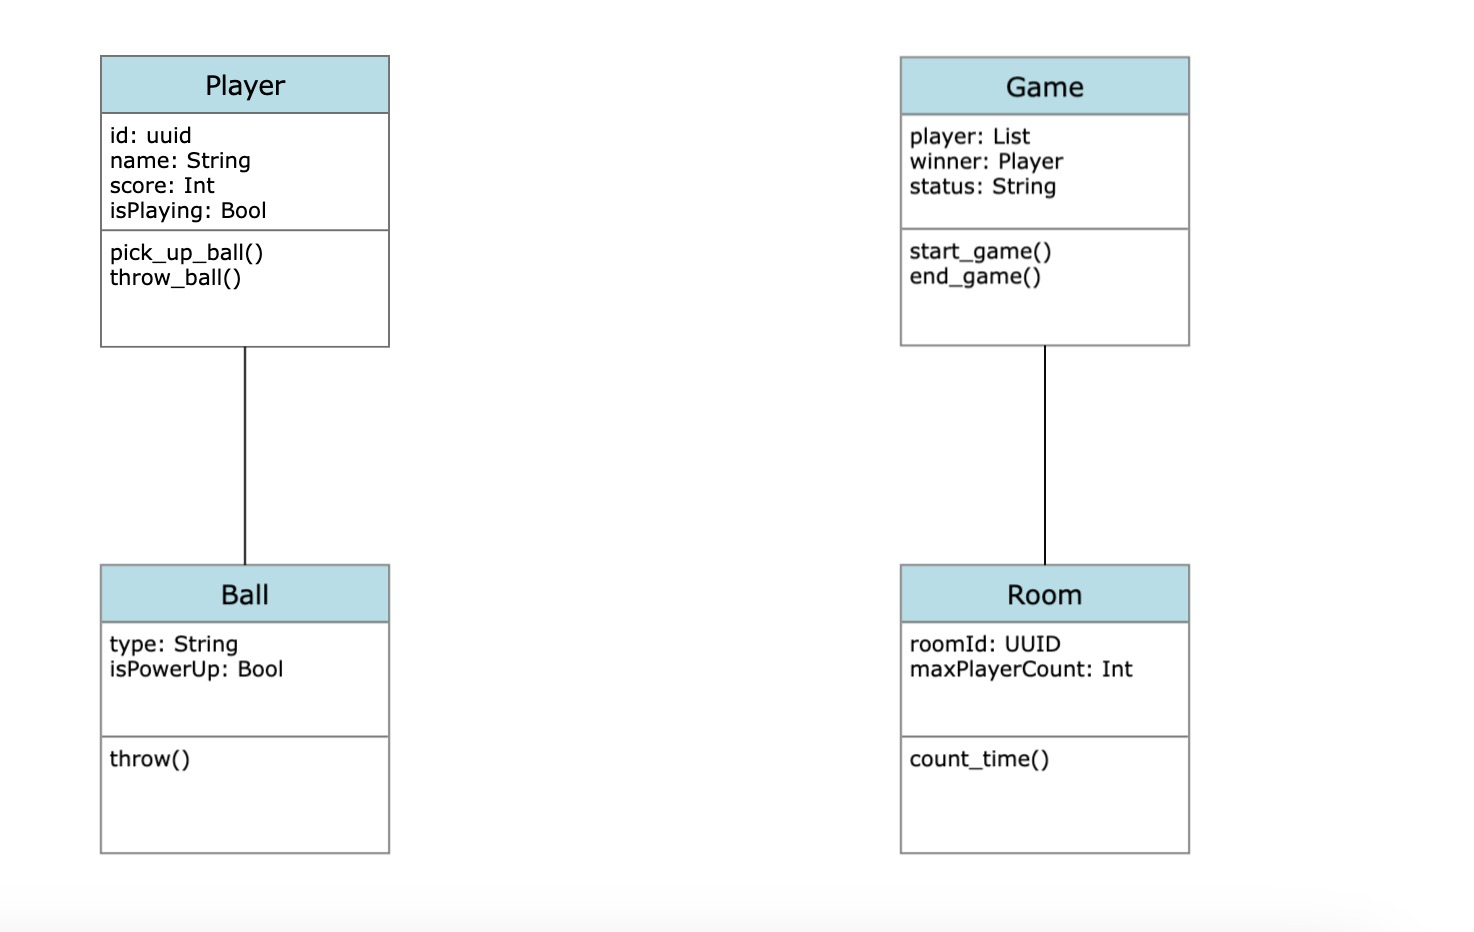
\includegraphics[scale=0.9]{images14.png}
\caption{Sequence Diagram}
\label{Sequence Diagram}
\end{figure}

\clearpage
\justifying
\setlength{\parindent}{4em}
\setlength{\parskip}{0.5em}
\renewcommand{\baselinestretch}{1.5}
\normalsize
\subsection{ Class Diagram}
Class diagram describes the structure of a system by showing the system’s classes, Their
attributes, and the relationships among the classes. Proposed system contains five different 
types of classes and each posses their own attributes and methods. Main Classes of the 
proposed system are NDSRRC, FP Tree, Apriory, Sanitised DB each have different 
functionalities.
\vspace{1.5cm}
\begin{figure}[h]
\centering
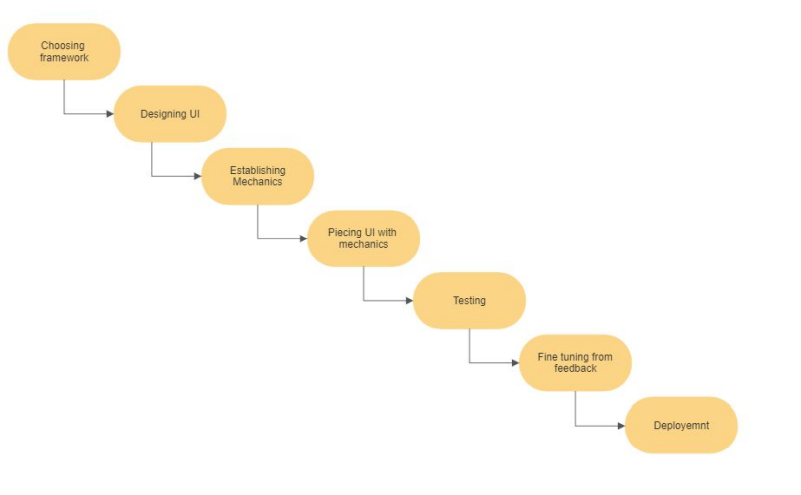
\includegraphics[scale=0.9]{ Class Diagram.png}
\caption{ Class Diagram
}
\label{ Class Diagram
}
\end{figure}


\clearpage
\justifying
\setlength{\parindent}{4em}
\setlength{\parskip}{0.5em}
\renewcommand{\baselinestretch}{1.5}
\normalsize
\subsection{ Entity Relationship Diagrams}
Class diagram describes the structure of a system by showing the system’s classes, Their
attributes, and the relationships among the classes. Proposed system contains five different 
types of classes and each posses their own attributes and methods. Main Classes of the 
proposed system are NDSRRC, FP Tree, Apriory, Sanitised DB each have different 
functionalities.
\vspace{1.5cm}

\clearpage
\centering
\section{ Project Estimation and Project Plan}
\justifying
\setlength{\parindent}{4em}
\setlength{\parskip}{0.5em}
\renewcommand{\baselinestretch}{1.5}
\normalsize In this chapter we are going to have an overview about how much time does it took to complete each task like- Preliminary Survey Introduction and Problem Statement, Literature Survey, Project Statement, Software Requirement and Specification, System Design, Partial Report Submission, Architecture Design, Implementation, Deployment, Testing, Paper Publish, Report Sub- mission and etcetera. This chapter also focuses on the stakeholder list which gives information about project type, customer of the proposed system, user and project member who developed the system.

% \subsection{PROJECT ESTIMATES}


\subsection{RISK MANAGEMENT}
\justifying
\setlength{\parindent}{4em}
\setlength{\parskip}{0.5em}
\renewcommand{\baselinestretch}{1.5}
\vspace{0.1cm}
\begin{enumerate}
\item In appropriate dataset -To overcome this risk we are trying to use a well organized and complete dataset.
\item Security- To overcome and improve security we use multilevel security like access permissions of users.

\end{enumerate}
\subsubsection{Risk Identification}
\justifying
\setlength{\parindent}{4em}
\setlength{\parskip}{0.5em}
\renewcommand{\baselinestretch}{1.5}
\vspace{0.1cm}
\begin{enumerate}
\item Are end-users enthusiastically committed to the project and the sys- tem/product to be built?
Ans-Not known at this time.
\item Are requirements fully understood by the software engineering team and its customers?
Ans-Yes
\item Does the software engineering team have the right mix of skills? Ans-yes
\item Is the number of people on the project team adequate to do the job? Ans-Not applicable
\item Do all customer/user constituencies agree on the importance of the project and on the requirements for the system/product to be built?
Ans-Not applicable
\end{enumerate}


\subsubsection{Risk Analysis}
\justifying
\setlength{\parindent}{4em}
\setlength{\parskip}{0.5em}
\renewcommand{\baselinestretch}{1.5}
\vspace{0.1cm}
\normalsize
The risks for the Project can be analyzed within the constraints of time and quality.Risk analysis for a malware detection system using SVM involves assessing potential vulnerabilities, threats, and potential impacts. Here's an overview of the risk analysis process:
\begin{itemize}
\item \textbf{Identify system vulnerabilities:} Identify the vulnerabilities in the malware detection system that could be exploited by attackers. This could include weaknesses in the SVM implementation, data storage, network communication, or any other component of the system.
\item \textbf{Threat identification:}: Identify potential threats that the system may face. This can include external threats, such as attackers attempting to bypass the detection system or exploit vulnerabilities, as well as internal threats, such as insider attacks or unintentional misuse of the system.
\item \textbf{Impact assessment: } Evaluate the potential impact of a successful attack or system failure. Consider the consequences in terms of data compromise, system downtime, financial losses, reputational damage, or any other relevant factors. This step helps prioritize risks based on their potential impact.
\item \textbf{Risk evaluation:} Combine the impact and likelihood assessments to determine the level of risk associated with each identified threat. This can be done by assigning risk levels, such as low, medium, or high, or by using a numerical risk scoring system. This step helps prioritize risks for mitigation efforts.
\item \textbf{Risk mitigation :}Develop strategies and measures to mitigate the identified risks. This may include implementing security controls, applying patches and updates, enhancing system monitoring and logging, conducting regular security assessments, or training system users to minimize human errors.
\item \textbf{Monitoring and review:} Regularly monitor the malware detection system and review the effectiveness of implemented risk mitigation measures. Stay updated on the evolving threat landscape and adjust risk mitigation strategies accordingly.
It's important to note that risk analysis should be an ongoing process, continuously adapted to address emerging threats and changes in the system and its environment. Regular risk assessments and updates to the malware detection system are essential to maintain a robust security posture.

\end{itemize}
\vspace{14cm}
\subsubsection{Risk Mitigation Risk Monitoring and Risk Management}
\justifying
\setlength{\parindent}{4em}
\setlength{\parskip}{0.5em}
\renewcommand{\baselinestretch}{1.5}

\normalsize
\vspace{1cm}

\vspace{14cm}
\subsection{PROJECT SCHEDULE}

\justifying
\setlength{\parindent}{4em}
\setlength{\parskip}{0.5em}
\renewcommand{\baselinestretch}{1.5}
\subsubsection{Project Task Set}
\normalsize
Major Tasks in the Project stages are:
\begin{enumerate}
\item Task 1: correctness
\item Task 2: availability
\item Task 3: integrity
\end{enumerate}
\vspace{0.1cm}


\vspace{14cm}
\subsection{Timeline Chart}
\justifying
\setlength{\parindent}{4em}
\setlength{\parskip}{0.5em}
\renewcommand{\baselinestretch}{1.5}

\vspace{1cm}











\clearpage


\centering
\section{OTHER SPECIFICATION}

\justifying
\setlength{\parindent}{4em}
\setlength{\parskip}{0.5em}
\renewcommand{\baselinestretch}{1.5}

\vspace{0.5cm}
\normalsize
\subsection{  ADVANTAGES}
\begin{itemize}
\item The main advantage of our music recommendation system is to provide 
suggestions to the users that fit the user's emotions.\\
\item The analysis of the facial expression/user emotion may lead to understanding the 
current emotional state of the user
\end{itemize}

\vspace{1.5cm}
\normalsize
\subsection{  APPLICATIONS}
\begin{itemize}
\item This system helps user to play songs automatically according to their mood.\\
\item Redirection of page to the music website once song is played.

\end{itemize}
\clearpage

\centering
\section{RESULT}

\justifying
\setlength{\parindent}{4em}
\setlength{\parskip}{0.5em}
\renewcommand{\baselinestretch}{1.5}
\vspace{1cm}



\vspace{1cm}


\vspace{1.5cm}


\vspace{1cm}


\vspace{1.5cm}


\vspace{1cm}


\vspace{1cm}


\vspace{1.5cm}


\vspace{1cm}

\clearpage
\centering
\section{TESTING}
\justifying
\setlength{\parindent}{4em}
\setlength{\parskip}{0.5em}
\renewcommand{\baselinestretch}{1.5}
\normalsize
\subsection{ Introduction}
\hspace{1.7 cm}Testing is an important part of software development life cycle. It is performed to ensure 
quality of the developed system. Testing includes a set of investigative activities that can be 
planned in advance and conducted systematically, to assure the stakeholder that system 
fulfils all the requirements gathered during requirement gathering phase. Software testing is 
one of the key elements in software projects that is often referred to as verification and 
validation. Verification refers to the set of activities that ensure that software correctly 
implements specified functionality. Validation refers to a set of activities built around 
traceability matrix which ensure that the functionality implemented by the system is 
traceable to customer requirements

Tests are the individual tests specified in a test plan document. Each test is typically 
described by
\begin{itemize}
\item An initial system state.
\item A set of actions to be performed.
\item The expected results of the test.
\end{itemize}

\subsection{ Implementation}
\justifying
\setlength{\parindent}{4em}
\setlength{\parskip}{0.5em}
\renewcommand{\baselinestretch}{1.5}
\normalsize

Test cases are planned in accordance to the test process and documented with detailed test 
descriptions. These test cases use cases based on projected operational mission scenarios. 
The testing process also includes stress or load testing for stability purpose (i.e., at 95% CPU 
use, system stability is still guaranteed. The test process thoroughly tests the interfaces and 
modules. Software testing includes a traceable white box testing, black box testing and other 
test processes verifying implemented software against design documentation and 
requirements specified.


\subsection{Objective
}
\justifying
\setlength{\parindent}{4em}
\setlength{\parskip}{0.5em}
\renewcommand{\baselinestretch}{1.5}
\normalsize

The software test plan (STP) is designed to test each module to measure its performance, to 
uncover bugs in the system, to set aright any flaws in logic that may be present, and to check 
logical flow from one module to another within system.
\begin{itemize}
\item All field entries must work properly.
\item Pages must be activated from the identified link.
\item The entry screen, messages and responses must not be delayed.

\end {itemize}


\subsection{Testing Strategy
}
\justifying
\setlength{\parindent}{4em}
\setlength{\parskip}{0.5em}
\renewcommand{\baselinestretch}{1.5}
\normalsize

A strategy outlines what to plan, and how to plan it. A successful strategy is your guide 
through change, and provides a firm foundation for ongoing improvement. Unlike a plan, 
which is obsolete from the point of creation, a strategy reflects the values of an organization 
- and remains current and useful. When an organization tests its products or its tools, it tries 
to compare them against its expectations and values. By its nature, testing introduces change 
as problems are identified and resolved. A test strategy is necessary to allow these two 
impulses to work together. Furthermore, testing can never be said to be ‘complete’, and a 
core skill in testing is the justified management of conflicting demands; without a strategy, 
these judgements will be inconsistent to the point of failure.\\
Software development is a creative process. A test strategy is a vital enabler to this process 
keeping focus on core values and consistent decision-making to help achieve desired goals 
with best use of resource. 

\subsection{ Types of Testing:
}
\justifying
\setlength{\parindent}{4em}
\setlength{\parskip}{0.5em}
\renewcommand{\baselinestretch}{1.5}
\normalsize

\hspace{1.7 cm} 1. White Box Testing: A level of white box test coverage is specified that is ap propriate for 
the software being tested. The white box and other testing uses automated tools to instrument 
the software to measure test coverage.

2. Black Box Testing: A black box test of integration builds includes functional, interface, 
error recovery, stress and out-of-bounds input testing. All black box software tests are traced 
to control requirements. In addition to static requirements, a black box of a fully integrated 
system against scenario sequences of events is designed to model field operation. 
Performance testing for systems is integrated as an integral part of the black box test process.


\subsection{ Unit Testing
}
\justifying
\setlength{\parindent}{4em}
\setlength{\parskip}{0.5em}
\renewcommand{\baselinestretch}{1.5}
\normalsize

Unit testing is used to check the execution path of the module, function, and procedure of 
the system. Test is conducted with the help of normal data and abnormal data. This testing 
includes the different factors like statement coverage, branch coverage, loop processing, 
abnormality, and circulation etc. With the help of this Unit testing we check that all the 
statement in the code is executed or not so it avoids the dead code statement. It checks all 
the branches and execution path of the code. It ensures that all the internal method of 
program are executed and properly integrated with program.

Unit testing involves the design of test cases that validate that the internal program logic is 
functioning properly, and that program inputs produce valid outputs. All decision branches 
and internal code flow should be validated. It is the testing of individual software units of 
the application .it is done after the completion of an individual unit before integration. This 
is a structural testing, that relies on knowledge of its construction and is invasive. Unit tests 
perform basic tests at component level and test a specific business process, application, 
and/or system configuration. Unit tests ensure that each unique path of a business process 
performs accurately to the documented specifications and contains clearly defined inputs 
and expected results.

\subsection{Integrated system}
\justifying
\setlength{\parindent}{4em}
\setlength{\parskip}{0.5em}
\renewcommand{\baselinestretch}{1.5}
\normalsize

In integrated testing, all the modules are checked together to ensure that all the modules are 
executing together according to the program specification. Once all the mod ules have been 
tested individually, the most legitimate question can be asked is that when all the modules 
are working properly, why there is need of integrated testing.

The answer is, though all modules are working properly problem may occur while interfacing 
individual module. Testing is event driven and is more concerned with the 
basic outcome of screens or fields. Integration tests demonstrate that although the components 
were individually satisfaction, as shown by successfully unit testing, the combination of 
components is correct and consistent. Integration testing is specifically aimed at exposing the 
problems that arise from the combination of components.

\subsection{ Functional test}
\justifying
\setlength{\parindent}{4em}
\setlength{\parskip}{0.5em}
\renewcommand{\baselinestretch}{1.5}
\normalsize

Functional tests provide systematic demonstrations that functions tested are available as 
specified by the business and technical requirements, system documentation, and user 
manuals. Functional testing is centered on the following items: Valid Input: identified classes 
of valid input must be accepted. Invalid Input: identified classes of invalid input must be 
rejected. Functions: identified functions must be exercised. Output: identified classes of 
application outputs must be exercised. Systems/Procedures: interfacing systems or procedures 
must be invoked.

Organization and preparation of functional tests is focused on requirements, key functions, or 
special test cases. In addition, systematic coverage pertaining to identify Business process 
flows; data fields, predefined processes, and successive processes must be considered for 
testing. Before functional testing is complete, additional tests are identified and the effective 
value of current tests is determined.




\clearpage


\centering
\section{Test Cases}
\justifying
\setlength{\parindent}{4em}
\setlength{\parskip}{0.5em}
\renewcommand{\baselinestretch}{1.5}
\normalsize
\subsection{GUI Test Cases}


\vspace{1cm}
\clearpage

\subsection{Registration Test Cases}


\vspace{1cm}
\clearpage

\subsection{Login Test Case}


\vspace{1cm}
\clearpage

\subsection{System Test Cases}

\vspace{1cm}
\clearpage


% start conclusion
\centering
\section{CONCLUSION }
\justifying
\setlength{\parindent}{4em}
\setlength{\parskip}{0.5em}
\renewcommand{\baselinestretch}{1.5}
\normalsize

\hspace{1.7cm}The proposed work presents facial expression recognition system to play a song according 
to the expression detected and classify music Type. It uses CNN approach to extract features. We 
are Developing a system to recognize user emotion based on facial expression using Python. We 
Integrate the python code into the web service and play the music based on the facial expression 
like happy, sad, or neutral. It is very good entertainment for the users. Emotion recognition using 
facial expressions is one of the important topics of research and has gathered much attention in the 
past. The problem of emotion recognition with the help of image processing algorithms has been 
increasing day by day. Researchers are continuously working on ways to resolve this using different 
kinds of features and image processing methods.\\
\vspace{15cm}
% end of conclusion


\centering
\Large\textbf{ANNEXURE A }

\centering

\Large\textbf{APPENDIX A}\\
\justifying
\setlength{\parindent}{4em}
\setlength{\parskip}{0.5em}
\renewcommand{\baselinestretch}{1.5}
\normalsize
\raggedright\textbf{What is P?}
\begin{itemize}
\item P is set of all decision problems which can be solved in polynomial time by a
deterministic.\\
\item  Since it can be solved in polynomial time, it can be verified in polynomial time.\\
\item  P is a subset of NP.
\end{itemize}

\textbf{P:}

A novel abstractive multi-document summarization system based on chunk-graph (CG) and
recurrent neural network language model (RNNLM). A CG which is basedon word-graph is 
constructed to organize all information in a sentence cluster, CG can reduce the size of graph 
and keep more semantic information than word-graph. System outperforms all baseline systems 
and reach the state-of-art systems, and thesystem with CG can generate better summaries than
that with ordinary word-graph.



\vspace{1cm}

\textbf{What is NP?
}

NP means we can solve it in polynomial time if we can break the normal rulesof step-by-step
computing.

\textbf{What is NP Hard?}

A problem is NP-hard if an algorithm for solving it can be translated into onefor solving
any NP-problem (nondeterministic polynomial time) problem. NP-hard therefore means at
least as hard as any NP-problem, although it might, in fact, beharder.

\textbf{Np-Hard:
}

A CG which is based on word-graph is constructed to organize all information in a sentence 
cluster, CG can reduce the size of graph and keep more semantic informa-tion than word-graph. 
We use beam search and character-level RNNLM to generatereadable and informative summaries
from the CG for each sentence cluster, RNNLMis a better model to evaluate sentence linguistic
quality than n-gram language model.the system with CG can generate better summaries than that 
with ordinary word- graph.



\vspace{1cm}

\textbf{What is NP-Complete?
}
\begin{itemize}
\item Since this amazing N computer can also do anything, a normal computer can, weknow 
that P problems are also in NP.
\item So, the easy problems are in P (and NP), but the really hard ones are only in
NP, and they are called NP-complete.
\item It is like saying there are things that People can do (P), there are things that Super 
People can do (SP), and there are things only Super People can do (SP- complete).
\end{itemize}
\textbf{NP-Complete:}

As our system is in developing state so we can’t say that our system is currently inNP
complete state

Ideas of pattern-growth in uncertain environment:

The ideas of pattern-growth in uncertain environment, two alternative algorithms aredesigned to 
discover all the STP candidates with support values for each user. That provides a trade-off 
between accuracy and efficiency. The user-aware rare pattern concerned here is a new concept 
and a formal criterion must be well defined, so thatit can effectively characterize most of
personalized and abnormal behaviors of Inter-net users.



\vspace{1cm}



% end of appendix

\centering
\Large\textbf{ANNEXURE B}

\centering

\Large\textbf{APPENDIX B}\\
\justifying
\setlength{\parindent}{4em}
\setlength{\parskip}{0.5em}
\renewcommand{\baselinestretch}{1.5}
\normalsize
\raggedright\textbf{Details of paper publication:} international Journal for Research in Applied Science and Engineering Technology(IJRASET)

\vspace{1cm}


\vspace{0.1cm} 






\vspace{15 cm}

\clearpage


\centering
\Large\textbf{ANNEXURE C}

\centering

\Large\textbf{APPENDIX C}\\
\justifying
\setlength{\parindent}{4em}
\setlength{\parskip}{0.5em}
\renewcommand{\baselinestretch}{1.5}
\large
\raggedright\textbf{Plagarism Report:}
\vspace{1cm}

\begin{figure}[h]
\centering
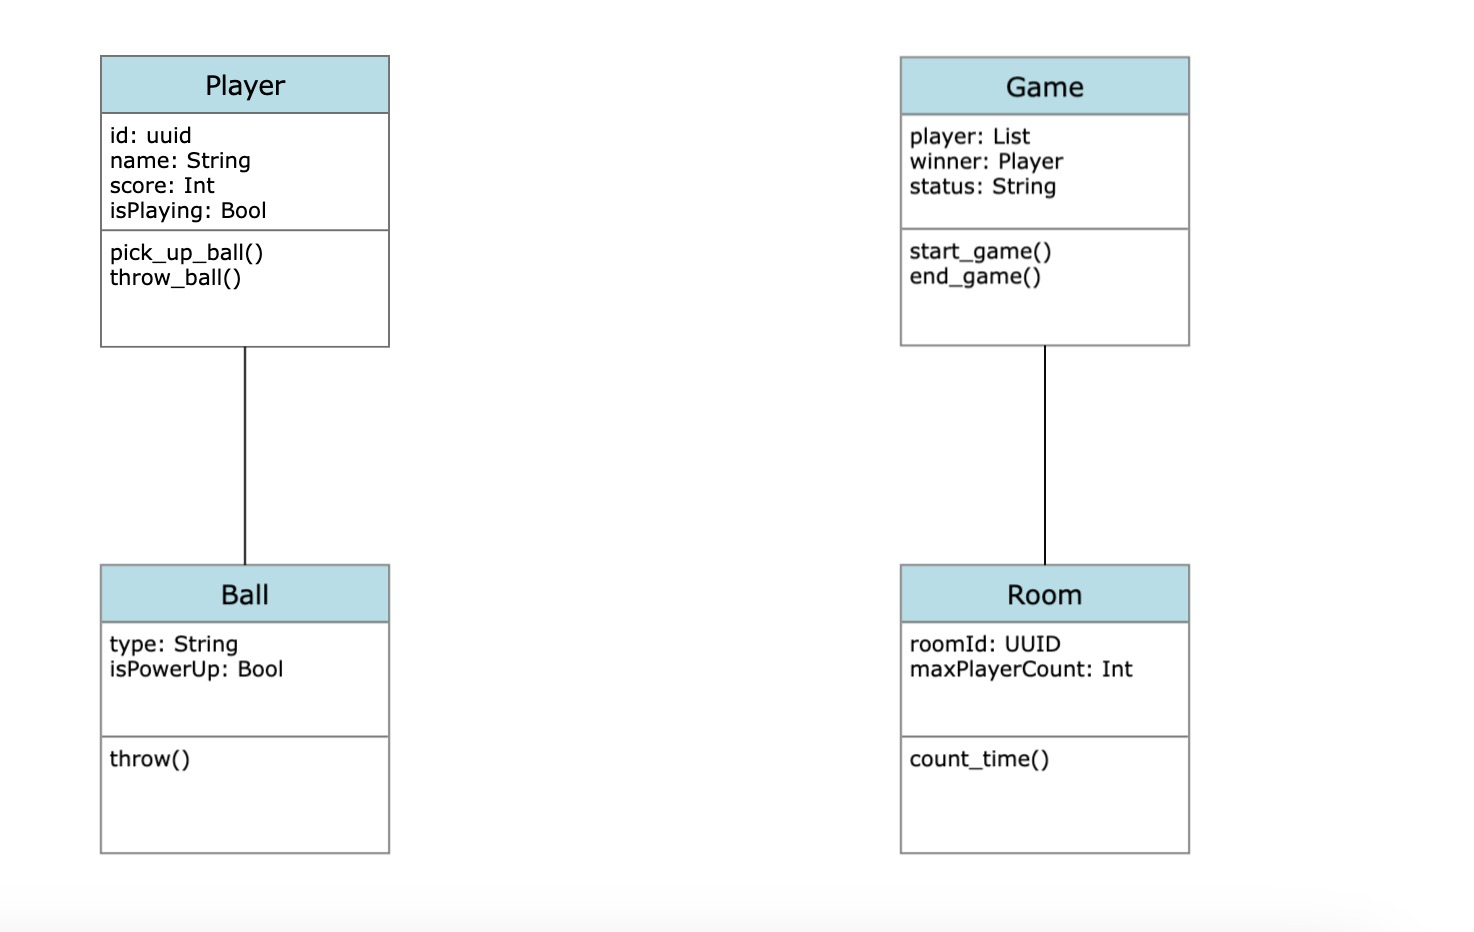
\includegraphics[scale=0.9]{images14.png}

\end{figure}
\vspace{15 cm}


% start of References
\centering
\Large\textbf{REFERENCES}
\justifying
\setlength{\parindent}{4em}
\setlength{\parskip}{0.5em}
\renewcommand{\baselinestretch}{1.5}
\normalsize

\begin{enumerate}


\item Vincenzo Moscato, Antonio Picariello and Giancarlo Sperli. An Emotional Recommender 
System for Music. October 01,2020 at 17:32:18 UTC from IEEE Xplore.

\item Ahlam Alrihaili, Alaa Alsaedi, Kholood Albalawi, Liyakathunisa Syed. Music  
Recommender System for users based on Emotion Detection through Facial Features. une 
22,2020 at 07:44:06 UTC from IEEE Xplore.

\item Metilda Florence, M Uma. Emotional Detection and Music Recommendation System based 
on User Facial Expression. IOP Conf. Series: Materials Science and Engineering 912 
(2020) 062007.

\item Sushmita G. Kambale, Asso. Prof. A.H. Kulkarni. Facial Expression based Music Player. 
Conference on Advances in Computing, Communications and Informatics (ICACCI), 
Sept. 21-24, 2016.

\item B. Naren Sai, D. Sai. Vamshi, Piyush Pogakwar, V. Seetharama Rao, Y. Srinivasulu. 
Music Recommendation System Using Facial Expression Recognition Using Machine 
Learning. ISSN: 2321-9653; IC Value: 45.98; SJ Impact Factor: 7.538 Volume 10 Issue 
VI June 2022.
\item Ziyang Yu1, Mengda Zhao1, Yilin Wu1, Peizhuo Liu1, Hexu Chen, Research On 
Automatic Music Recommendation Algorithm Based On "Facial Micro-Expression 
Recognition”, Proceedings Of The 39th Chinese Control Conference July 27-29, 2020. 
\item Dr. Sunil Bhutada, Ch. Sadhvika, Gutta.Abigna, P. Srinivas Reddy, "Emotion Based 
Music Recommendation System", Jeter April 2020. 
\item Mikhail Rumiantcev, Oleksiy Kiriyenko, "Emotion Based Music Recommendation 
System", Proceeding of the 26th Conference of Fruct Association.

\item Krupa K S, Kartikey Rai, Ambara G, Sahil Choudhury, "Emotion Aware Smart Music 
Recommender System Using Two Level CNN", Third International Conference On Smart 
Systems And Inventive Technology (Icssit 2020).



\end{enumerate}
%\subsubsection{WEB RESOURCES}
%\begin{enumerate}
%\item  \href{URL}{www.wikipedia.org}
%\item  \href{URL}{www.sciencedirect.com}
%\item  \href{URL}{www.slideshare.net}
%\end{enumerate}
\clearpage
%end of references


% seminar report documentation


\end{document}
